% Appendix B: Supplementary Material for Chapter 5
% Source: extracted from src/ch6_rnaanneal.tex

\begin{algorithm}[H]
  \caption{Sampling RNA secondary structures with \texttt{EternaFold}}
  \label{ch6:alg:eternafold-sampling}
  \begin{algorithmic}[1]
    \REQUIRE \texttt{example.fa} (input sequence);\\
    \texttt{N} (maximum number of samples, \texttt{5000})
    \STATE \texttt{mkdir -p eternafold}
    \STATE \texttt{EternaFold/src/contrafold sample example.fa} \\
    \ \texttt{--params EternaFold/parameters/EternaFoldParams.v1} \\
    \ \texttt{--nsamples N > eternafold/ef.ss}
  \end{algorithmic}
\end{algorithm}

\begin{algorithm}[H]
  \caption{Sampling RNA secondary structures with \texttt{LinearFold}}
  \label{ch6:alg:linearfold-sampling}
  \begin{algorithmic}[1]
    \REQUIRE \texttt{example.fa} (input sequence)
    \STATE \texttt{mkdir -p linearfold-v}
    \COMMENT {Vienna parameters}
    \STATE \texttt{mkdir -p linearfold-c}
    \COMMENT {CONTRAfold parameters}
    \STATE \texttt{cat example.fa | linearfold --zuker --delta 1000 -V | tail -n +5 | awk '\{print \$1\}' > linearfold-v/zuker.ss} \\
    \STATE \texttt{cat example.fa | linearfold --zuker --delta 1000       | tail -n +5 | awk '\{print \$1\}' > linearfold-c/zuker.ss}
  \end{algorithmic}
\end{algorithm}

\begin{algorithm}[H]
  \caption{Sampling RNA secondary structures with \texttt{LinearAliFold}}
  \label{ch6:alg:linearalifold-sampling}
  \begin{algorithmic}[1]
    \REQUIRE \texttt{example.fa} (input sequence);\\
    \texttt{N} (maximum number of samples, \texttt{20000})
    \STATE \texttt{mkdir -p linearalifold-v}
    \COMMENT {Vienna parameters}
    \STATE \texttt{mkdir -p linearalifold-bl}
    \COMMENT {BL* parameters}

    \STATE \texttt{cat example.fa | linearalifold.py -s N -e 1 > linearalifold-v/stochastic.ss}
    \STATE \texttt{cat example.fa | linearalifold.py -s N -e 2 > linearalifold-bl/stochastic.ss}
    \STATE \texttt{cat example.fa | linearalifold.py -p -B linearalifold-v/bpp.txt -M linearalifold-v/mea.ss -T linearalifold-v/threshknot.ss -C linearalifold-v/centroid.ss -e 1}
    \STATE \texttt{cat example.fa | linearalifold.py -p -B linearalifold-bl/bpp.txt -M linearalifold-bl/mea.ss -T linearalifold-bl/threshknot.ss -C linearalifold-bl/centroid.ss -e 2}
  \end{algorithmic}
\end{algorithm}

\begin{algorithm}[H]
  \caption{Conformational sampling with FARFAR2}
  \label{ch6:alg:rna_denovo}
  \begin{algorithmic}[1]
  \REQUIRE \texttt{SEQ} (input sequence);\\
  \texttt{DB} (secondary structure in dot-bracket notation)
    \STATE \texttt{rna\_denovo.default.linuxgccrelease} \\
    \ \texttt{-sequence SEQ} \COMMENT {From \texttt{example.fa} in Algorithms \ref{ch6:alg:eternafold-sampling}-\ref{ch6:alg:linearalifold-sampling}} \\
    \ \texttt{-secstruct DB} \COMMENT {\texttt{cat */*.ss | uniq} from Algorithms \ref{ch6:alg:eternafold-sampling}-\ref{ch6:alg:linearalifold-sampling}}\\
    \ \texttt{-nstruct 1} \\
    \ \texttt{-cycles 20000} \\
    \ \texttt{-minimize\_rna true} \\
    \ \texttt{-rna:denovo:rounds 10} \\
    \ \texttt{-rna:denovo:minimize:minimize\_bps true} \\
    \ \texttt{-rna:denovo:bps\_moves true}
  \end{algorithmic}
\end{algorithm}

\begin{algorithm}[H]
  \caption{Reference conformation preparation with FARFAR2}
  \label{ch6:alg:farfar-minimise}
  \begin{algorithmic}[1]
    \REQUIRE \texttt{SEQ} (input sequence);\\
    \texttt{REF} (reference PDB file)
    \STATE \texttt{rna\_denovo.default.linuxgccrelease} \\
    \ \texttt{-sequence \$(echo \$SEQ)} \COMMENT{lower‑case sequence} \\[-0.2em]
    \ \texttt{-secstruct '.....'} \COMMENT{all bases unpaired; equal to length of \texttt{\$SEQ}} \\[-0.2em]
    \ \texttt{-nstruct 1} \\[-0.2em]
    \ \texttt{-out:file:silent \$(dirname \$REF)/silent.out} \\[-0.2em]
    \ \texttt{-s \$REF} \COMMENT{experimental model} \\[-0.2em]
    \ \texttt{-minimize\_rna true} \\[-0.2em]
    \ \texttt{-rna:denovo:rounds 1} \\[-0.2em]
    \ \texttt{-out:overwrite true} \\[-0.2em]
    \ \texttt{-cycles 10000} \\[-0.2em]
    \ \texttt{-rna:denovo:minimize:minimize\_bps true}
  \end{algorithmic}
\end{algorithm}

\begin{algorithm}[H]
  \caption{Unsupervised selection of diverse candidate conformations}
  \label{ch6:alg:candidate-selection}
  \begin{algorithmic}[1]
    \REQUIRE FARFAR2 models $\{\mathbf{x}_i\}_{i=1}^{N}$; \\
    Density‐peaks parameter $Z{=}3$;\\
    Principal component range $d\!=\!2,3\ldots\,26$;\\
    Target count $K{=}200$
    \STATE Featurize each model $\mathbf{x}_i$ into a G-vector
    \FOR{$d \in \{2,3,\dots,26\}$}
      \STATE Project all G-vectors onto the first $d$ principal components
      \STATE Cluster the projection with \texttt{dadapy} (advanced density peaks, $Z{=}3$)
      \STATE Record the number of clusters obtained
    \ENDFOR
    \STATE Let $d^\ast$ be the dimension giving the maximum cluster count \COMMENT{see Fig.\,S\ref{ch6:fig:clusters_vs_d}}
    \STATE Re-cluster the $d^\ast$-dimensional data to obtain $\{\mathcal{C}_j\}_{j=1}^{M}$
    \FORALL{clusters $\mathcal{C}_j$}
      \STATE Sort conformations in $\mathcal{C}_j$ by ascending Rosetta score
    \ENDFOR
    \STATE Sort the clusters by the best Rosetta score among all conformations in each cluster
    \STATE $\mathcal{S} \leftarrow \varnothing$ \COMMENT{set of selected candidates}
    \WHILE{$|\mathcal{S}| < K$}
      \FOR{$j = 1$ \TO $M$}
        \IF{$\mathcal{C}_j \neq \varnothing$}
          \STATE Remove the top-scoring conformation $c$ from $\mathcal{C}_j$ and add $c$ to $\mathcal{S}$
          \IF{$|\mathcal{S}| = K$}
            \STATE \textbf{break}
          \ENDIF
        \ENDIF
      \ENDFOR
      \STATE Re-sort clusters by their current top-scoring conformation
    \ENDWHILE
    \RETURN $\mathcal{S}$ \COMMENT{200 candidate conformations}
  \end{algorithmic}
\end{algorithm}

\begin{algorithm}[H]
  \caption{Likelihood estimation for a thermodynamic map (diffusion model) using the Hutchinson trace estimator}
  \label{ch6:alg:diffusion-likelihood}
  \begin{algorithmic}[1]
    \REQUIRE Observed frame $\mathbf{u}_{0}\equiv (\mathbf{x}_0, U_0)^\top$ (data at $t_0\equiv t={0}$); \\
    Diffusion process $\mathcal{D}$ with time grid $\{t_{0}\!\!<\!\!t_{1}\!\!<\!\!\dots\!\!<\!\!t_{K}\}$; \\
    One–step map $\mathrm{STEP}_{t_{k}\!\rightarrow t_{k+1}} \colon \mathbf{u}\!\mapsto\!\mathbf{u}'$; \COMMENT{Neural network} \\
    Prior temperature $T$; \COMMENT{$T=1$ unless otherwise stated} \\
    Temperature-dependent prior density $q_T(\mathbf{u}_{t_K})\equiv \mathcal{N}(0,T) \times \mathcal{N}(0,1)$; \COMMENT{Different priors for $\mathbf{x}$ and $U$} \\
    Schedule of noise scales $\{\beta_{k}\}_{k=1}^{K}$; \\
    Number of Hutchinson probe vectors $M$
    \STATE $\mathbf{u}\leftarrow\mathbf{u}_{0}$  \COMMENT{state at the current time $t_{k}$}
    \STATE $\mathcal{G}\leftarrow[\,]$          \COMMENT{to store divergence $g_{k}$}
    \FOR{$k\;=\;0\;\mathbf{to}\;K-1$}
      \STATE Draw $M$ probe vectors
             $\bigl\{\mathbf{v}^{(m)}\bigr\}_{m=1}^{M}
                    \sim\mathcal{N}\bigl(\mathbf{0},\mathbf{I}\bigr)$
      \FORALL{probes $m=1,\dots,M$}
        \STATE $(\mathbf{u}'^{(m)},\mathbf{Jv}^{(m)})\;
               \leftarrow\;
               \mathrm{JVP}\Bigl(
                 \mathrm{STEP}_{t_{k}\!\rightarrow t_{k+1}},
                 \mathbf{u},\,
                 \mathbf{v}^{(m)}
               \Bigr)$ \COMMENT{Jacobian‐vector product}
      \ENDFOR
      \STATE $\displaystyle
             g_{k}\;\leftarrow\;
             \frac{1}{M}
             \sum_{m=1}^{M}
               \bigl\langle
                 \mathbf{Jv}^{(m)},\,\mathbf{v}^{(m)}
               \bigr\rangle$
             \COMMENT{Hutchinson trace estimate of $\nabla_{\!\mathbf{u}}\!\cdot\!\mathrm{STEP}$}
      \STATE Append $g_{k}$ to $\mathcal{G}$
      \STATE $\mathbf{u}\leftarrow\mathbf{u}'^{(1)}$ \COMMENT{all probes have the same output}
    \ENDFOR

    \STATE $\displaystyle
           \Delta \l_{pq}
           \leftarrow
           \operatorname{trapz}\bigl(\mathcal{G},\,
                                    \{\beta_{k}\}_{k=1}^{K}\bigr)$
           \COMMENT{trapezoidal integration on $(g_{k},\beta_{k})$}
    \STATE $\displaystyle
           \log q
           \leftarrow
           \log q_T\bigl(\mathbf{u}\bigr)$
           \COMMENT{prior log‐density at $t_{K}$ at temperature $T$}
    \STATE $\displaystyle
           \log p_{\theta}\bigl(\mathbf{u}_{0}\bigr)
           \leftarrow
           \log q + \Delta_{pq}$
    \RETURN $\log p_{\theta}(\mathbf{u}_{0})$
  \end{algorithmic}
\end{algorithm}

\begin{algorithm}[H]
  \caption{RNAnneal Score}
  \label{ch6:alg:rnanneal-score}
  \begin{algorithmic}[1]
    \REQUIRE  
    Log-likelihoods $\{L_{i}^{(\mathcal{F})}\}$;\\
    Feature sets $\mathcal{F}=\{\text{G-vector},\text{R-vector}\}\times\{\text{PCA},\text{SPIB}\}$;\\
    Component range $\mathcal{D}=2,3,\ldots,8$

    \STATE $\displaystyle L_{\min}\leftarrow\min_{i}L_{i}$,\quad 
           $\displaystyle\sigma_{L}\leftarrow\sqrt{\operatorname{Var}\{L_{i}\}}$
    \FORALL{frames $i$}
      \STATE $\displaystyle l_{i}\;\leftarrow\;
              {\bigl(L_{i}-L_{\min}\bigr)}\;
              {/\;\sigma_{L}}$ \COMMENT{subtract min and divide by SD}
    \ENDFOR
      \STATE Sort $\{l_{i}\}$ in ascending order
      \STATE Initialize lists $\mathcal{S} = [\,]$ and $\mathcal{L} = [\,]$
    \FORALL{confrmers $i$}
    
        \STATE $\mathcal{L}(i)\gets[\,]$
        \FORALL{feature-projection pairs $(v,f)\in\mathcal{F}$}
          \FORALL{dimensions $d\in\mathcal{D}$}
              \STATE Append $l_{i}^{(v,f,d)}$ to $\mathcal{L}(i)$
            \ENDFOR
          \ENDFOR
        \STATE Append {$\displaystyle\bar{s}_{i}
               = \frac{1}{|\mathcal{L}(i)|}\sum_{l\in\mathcal{L}(i)}l$} to ${\mathcal{S}}(i)$
               \COMMENT{{RNAnneal Score}}
       
      \ENDFOR
      \RETURN ${\mathcal{S}}(i)$
  \end{algorithmic}
\end{algorithm}

\begin{algorithm}[H]
  \caption{Interaction Entropy calculation}
  \label{ch6:alg:interaction-entropy}
  \begin{algorithmic}[1]
    \REQUIRE Ensemble of conformations $\{X_{1},\dots,X_{M}\}$;\\
             Nucleotides $i=1,\dots,N$; \\
             Prior weights $\{w_{1},\dots,w_{M}\}$ with $\sum_{j} w_{j}=1$; \\
             LW classification function $\mathrm{LW}(i,X_{j}) \rightarrow c \in \mathcal{C}$.
    \FORALL{nucleotides $i=1,\dots,N$}
      \STATE Initialize frequency table $f_{i}(c) \gets 0$ for all $c \in \mathcal{C}$
      \FORALL{conformations $j=1,\dots,M$}
        \STATE $c \gets \mathrm{LW}(i,X_{j})$
        \STATE $f_{i}(c) \gets f_{i}(c) + w_{j}$
      \ENDFOR
      \STATE $p_{i}(c) \gets f_{i}(c) / \sum_{c' \in \mathcal{C}} f_{i}(c')$ \COMMENT{Normalize}
      \STATE $H_{i} \gets -\sum_{c \in \mathcal{C}} p_{i}(c) \log_2 p_{i}(c)$
    \ENDFOR
    \RETURN $\{H_{i}\}_{i=1}^{N}$ \COMMENT{interaction entropies for all nucleotides}
  \end{algorithmic}
\end{algorithm}

\begin{algorithm}[H]
  \caption{Boltzmann‑weighted state ranking and representative selection}
  \label{ch6:alg:state-ranking}
  \begin{algorithmic}[1]
    \REQUIRE\ SPIB projections $\{\mathbf{x}_{i}\}$;\\
    State labels $\{y_{i}\}$;\\
    RNAnneal scores $\{s_{i}\}$;\\ Frame keys $\{f_{i}\}$;\\ Histogram grid size $(K=25,L=25)$;\\ Minimum population $N_{\min}=10$;\\ Pre‑filter count $k_{\mathrm{top}}=10$;\\ Report count $k_{\mathrm{rep}}=10$
    \STATE $\mathcal{F}\!\leftarrow\!\{(y_{i},\mathbf{x}_{i},s_{i},f_{i})\}$ 
    \STATE Group $\mathcal{F}$ by state label to obtain $\{\mathcal{F}_y\}$
    \STATE Discard states with $|\mathcal{F}_y|<N_{\min}$
    \STATE Compute the average score $\bar{s}_y $ for every surviving state
    \STATE Keep the $k_{\mathrm{top}}$ states with the lowest $\bar{s}_y$
    \STATE Initialise histogram $H$ on an $K\times L$ grid over 2D IB space
    \FORALL{frames $(y,\mathbf{x},s,f)\in\bigcup\mathcal{F}_y$}
      \STATE Increment $H$ at the bin containing $\mathbf{x}$ with $(s,y)$
    \ENDFOR
    \FORALL{occupied bins $(k,l)$}
      \STATE $\bar{s}_{kl}\!\leftarrow\!\text{mean score in bin }(k,l)$
      \STATE $w_{kl}\!\leftarrow\!\exp(-\bar{s}_{kl})$ \COMMENT{Boltzmann weight in bin $h_{kl}$}
      \STATE $y^\ast\!\leftarrow\!\arg\max_y\{\text{count of }y\text{ in }(k,l)\}$ \COMMENT{State assigned to bin $h_{kl}$}
      \STATE $W_{y^\ast}\!\leftarrow\!W_{y^\ast}+w_{kl}$ \COMMENT{Each bin $h_{kl}$ with state $y^\ast$ contributes $w_{kl}$ to the total state weight $W_{y^\ast}$}
    \ENDFOR
    \STATE $p_y\!\leftarrow\!W_y\,/\,\sum_{y'}W_{y'}$ \COMMENT{Normalize weights}
    \STATE Order states by $p_y$ (descending) to obtain $(y_{(1)},\dots,y_{(k_{\mathrm{rep}})})$
    \FOR{$r=1$ \TO $k_{\mathrm{rep}}$}
      \STATE $y\!\leftarrow\!y_{(r)}$
      \STATE $\mathcal{F}_y\!\leftarrow\!\{(s,f)\in\mathcal{F}_y\}$
      \STATE $f^\ast\!\leftarrow\!\arg\min_{(s,f)\in\mathcal{F}_y}\{s\}$ \COMMENT{representative frame}
      
      \STATE Record $\bigl(r,y,p_y,f^\ast\bigr)$
    \ENDFOR
    \RETURN\ Table of the $k_{\mathrm{rep}}$ most‑probable states with their representatives
  \end{algorithmic}
\end{algorithm}

\begin{figure*}
    \centering
    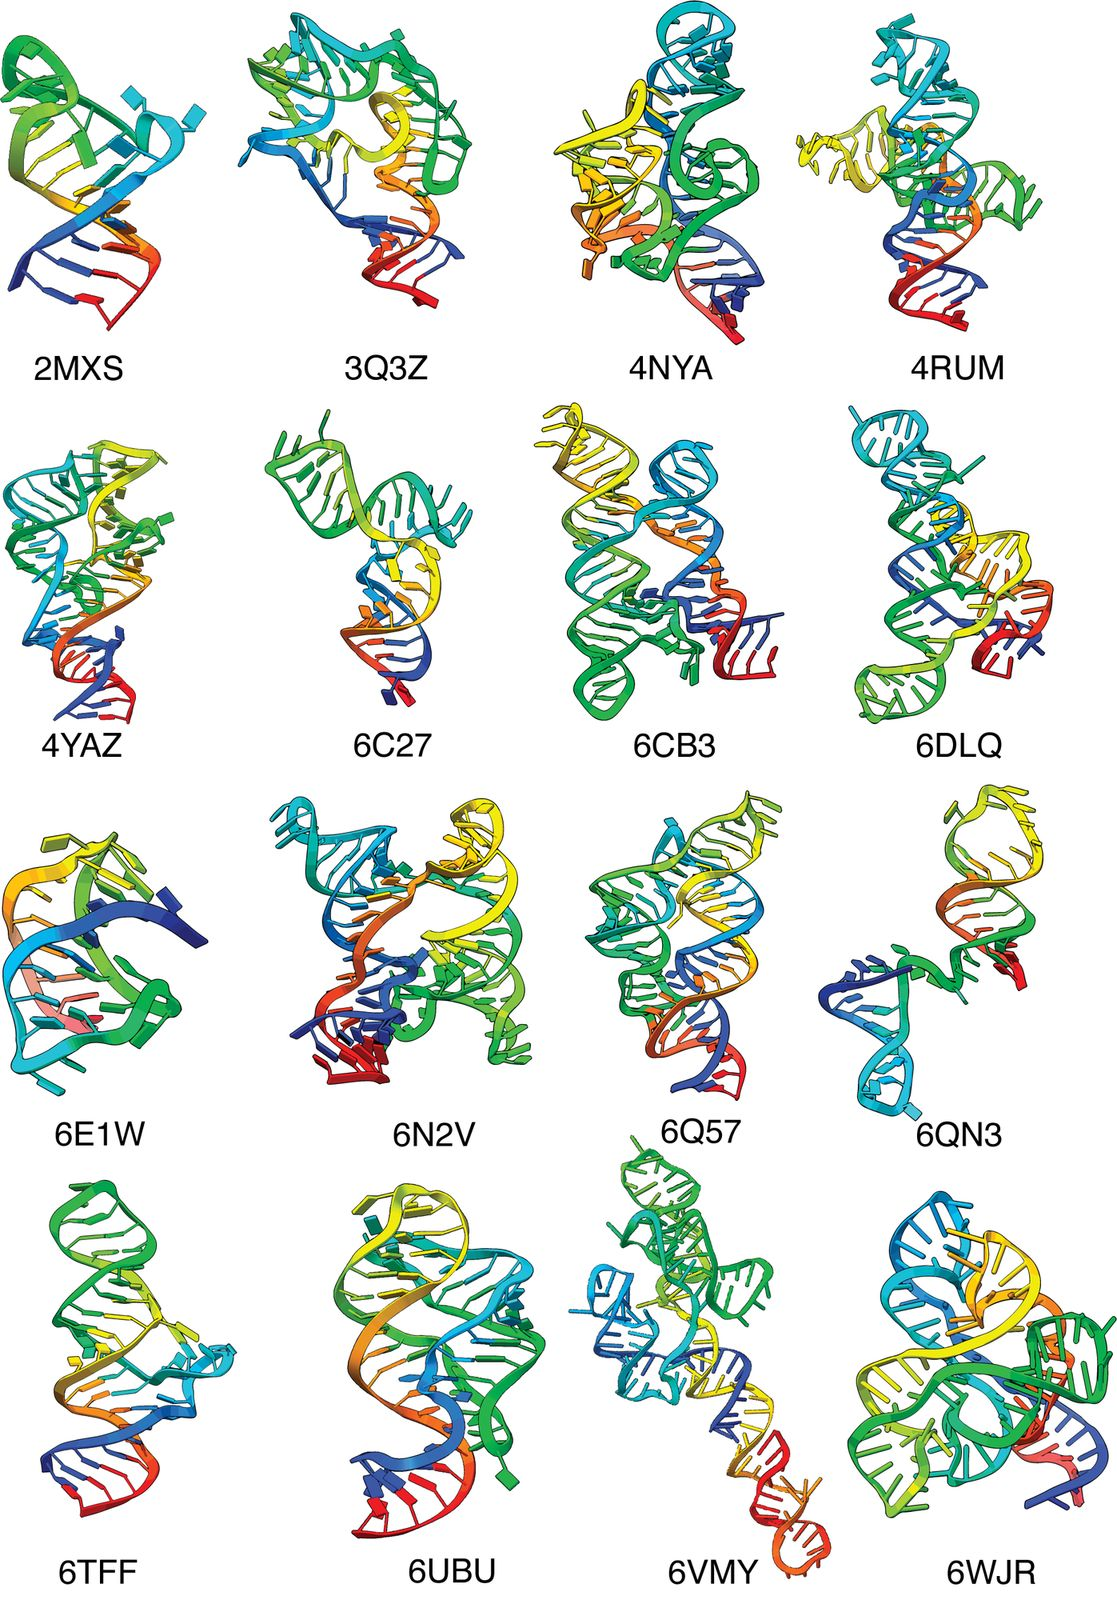
\includegraphics[
    width=0.7\textwidth
    ]{figures/ch6_all-representatives.jpg}
    \caption[Riboswitch reference ERCs labeled with PDB accession code.]{{\bf Riboswitch reference ERCs labeled with PDB accession code.}}
    \label{ch6:fig:all-representatives}%
\end{figure*}

\begin{figure}
    \centering
    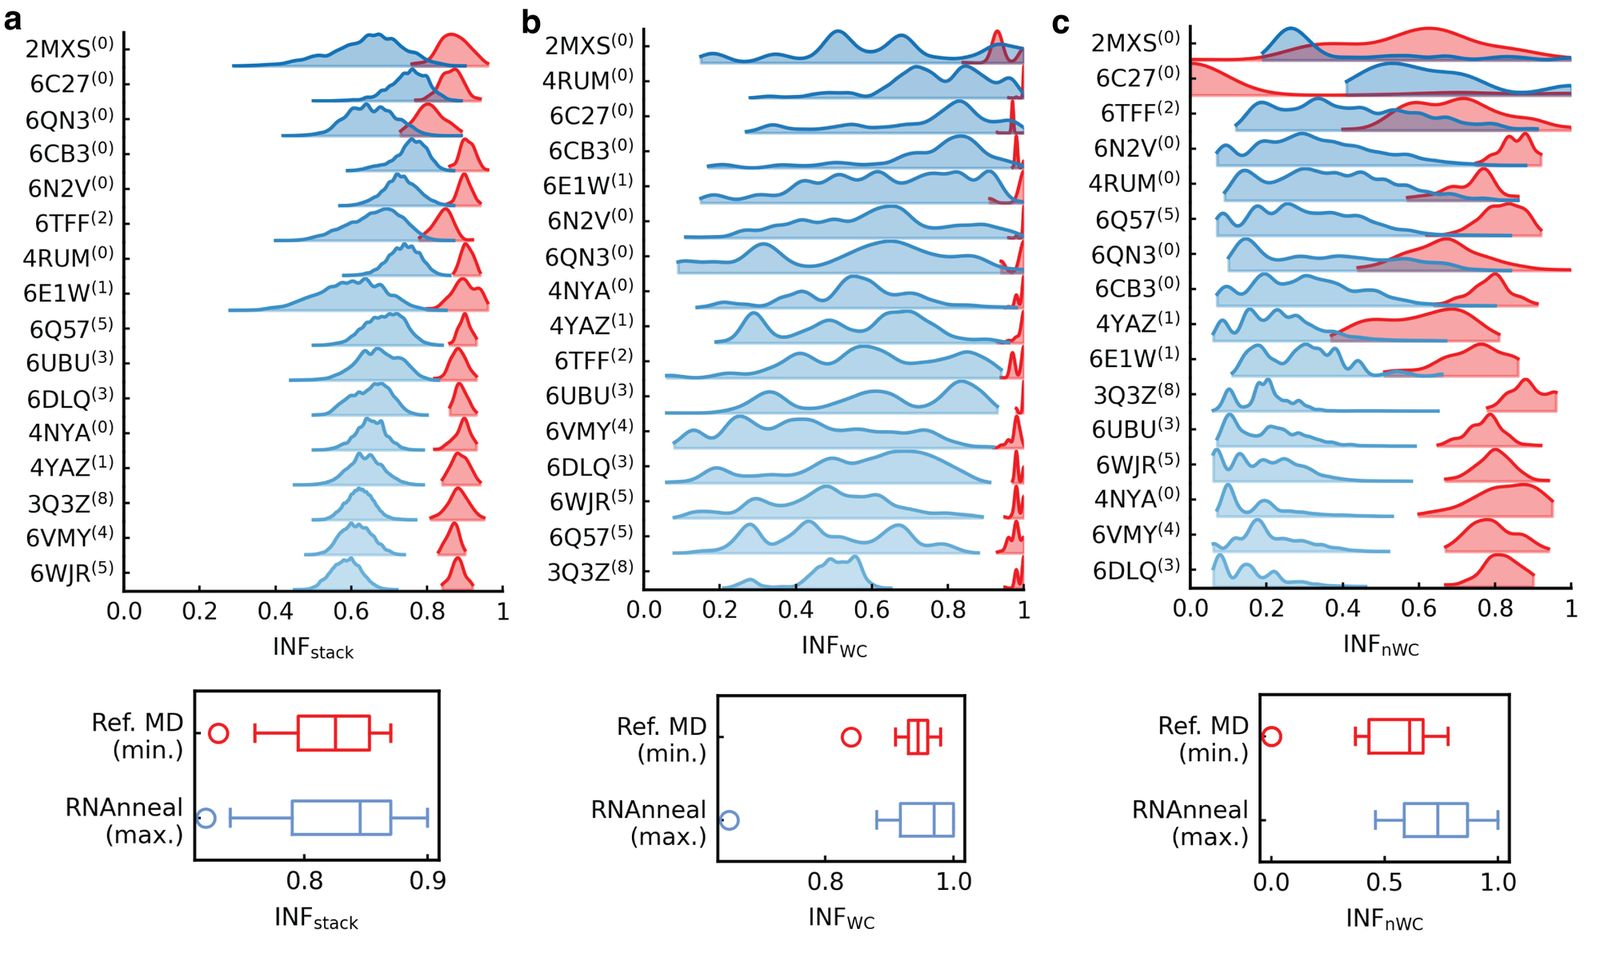
\includegraphics[
    width=0.9\textwidth
    ]{figures/ch6_stack-wc-nwc.jpg}
    \caption[Interaction Network Fidelity (INF) by interaction type.]{{\bf Interaction Network Fidelity (INF) by interaction type.} The INF is reported for {\textbf{a}.} stacking interactions (Median [IQR]; Ref. MD: 0.82 [$0.79-0.86$]; RNAnneal: 0.85 [$0.80-0.87$]),  {\textbf{b}.} Watson-Crick (WC) interactions (Ref. MD: 0.95 [$0.93-0.96$]; RNAnneal: 0.98 [$0.92-1.0$]), {\textbf{c}.} non-Watson-Crick (nWC) interactions (Ref. MD: 0.62 [$0.48-0.67$]; RNAnneal: 0.80 [$0.59-0.87$]). It is worth noting that the conformation with, e.g., the maximum $\mathrm{INF_{WC}}$, does not necessarily have the maximum $\mathrm{INF_{stack}}$ or $\mathrm{INF_{nWC}}$.}
    \label{ch6:fig:inf-detailed}%
\end{figure}

\begin{figure}
    \centering
    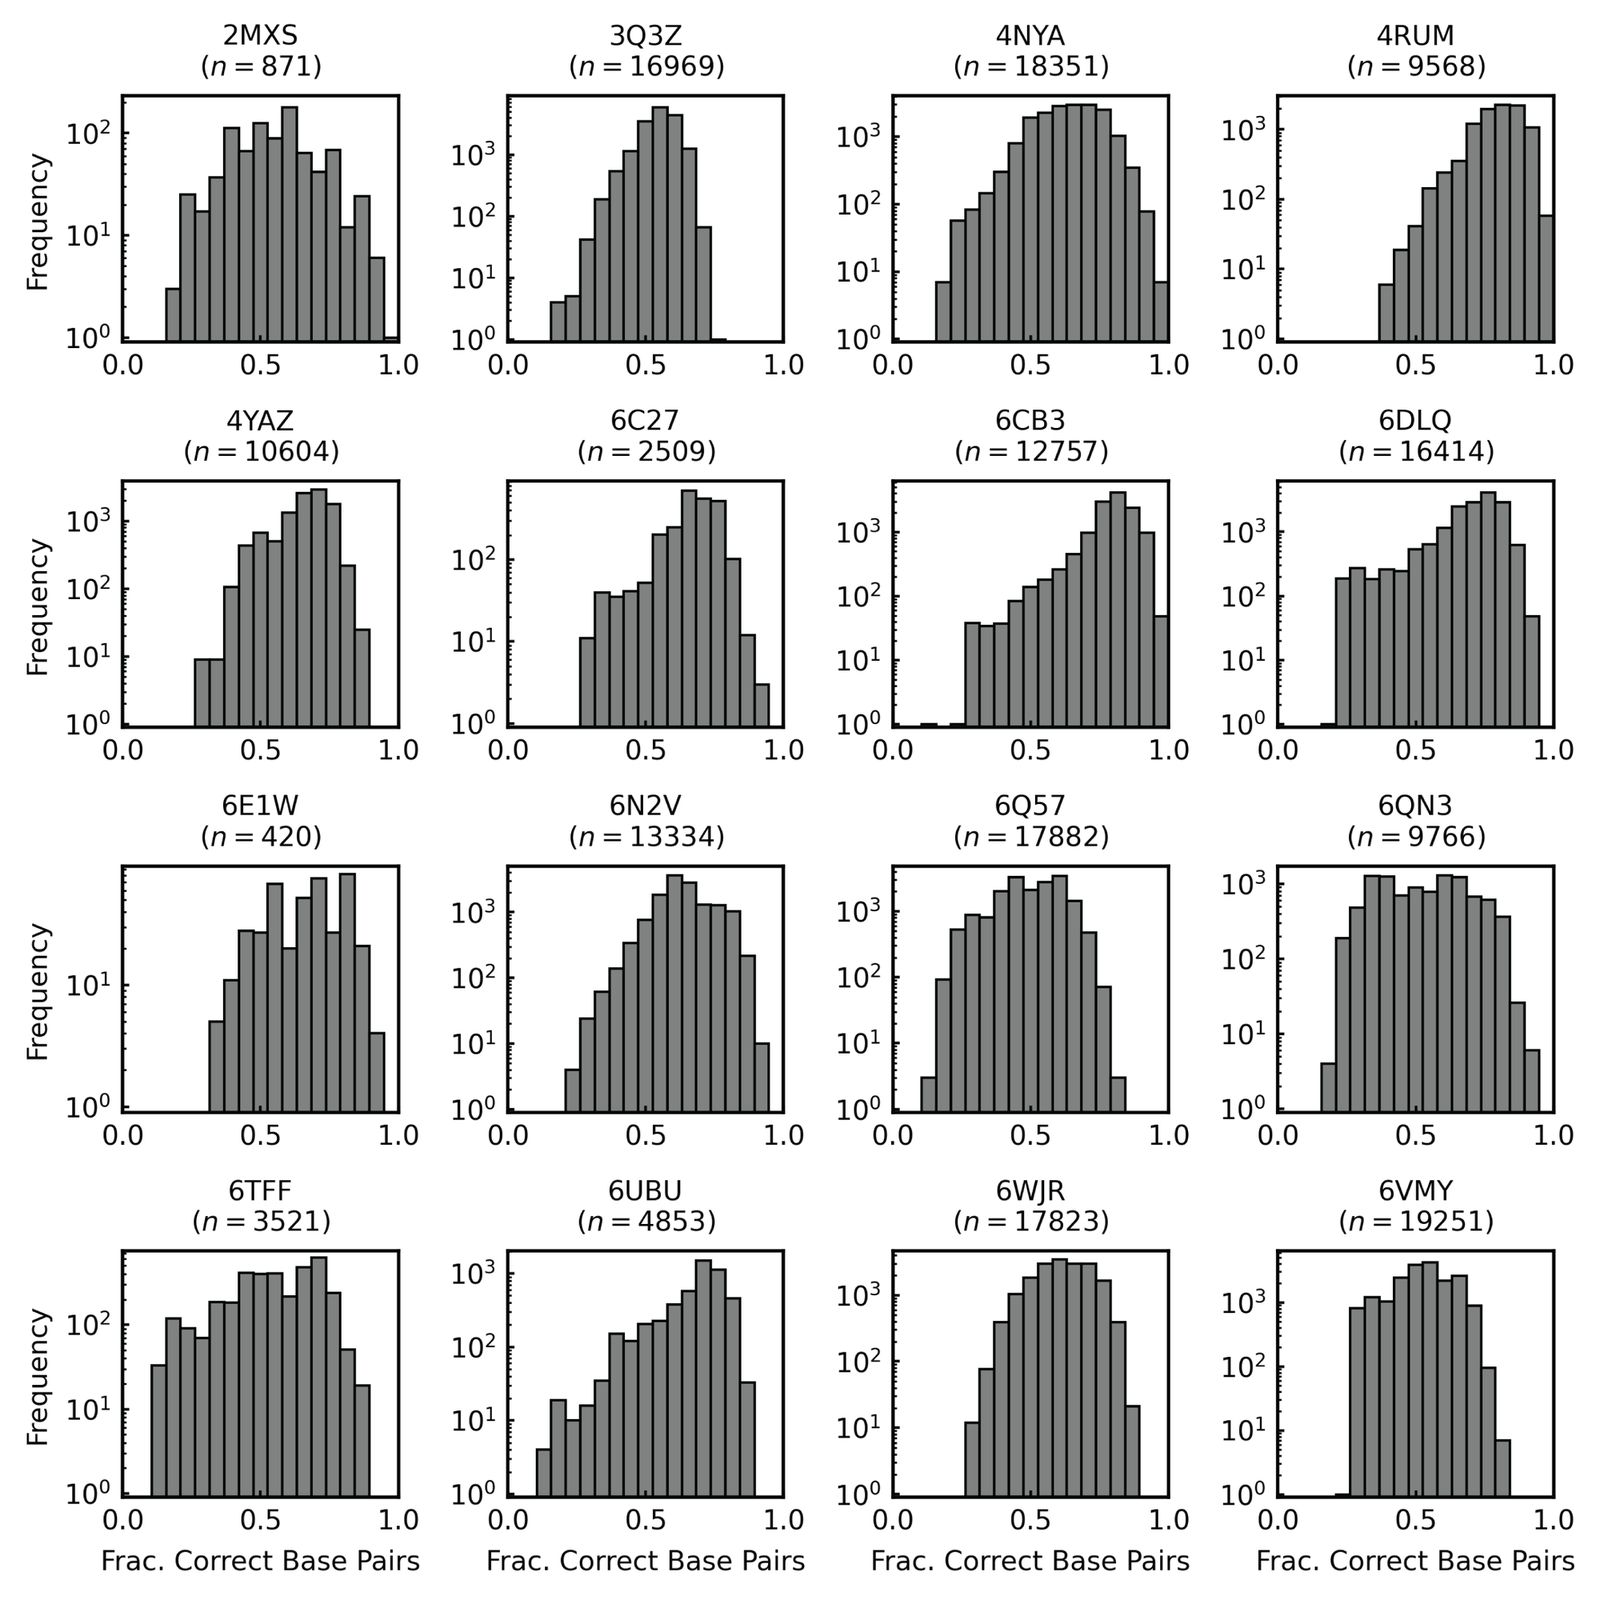
\includegraphics[
    width=\textwidth
    ]{figures/ch6_sec-struct-all.jpg}
    \caption[Evaluation of secondary structures predicted by EternaFold, LinearFold, and LinearAlifold.]{{\bf Evaluation of secondary structures predicted by EternaFold, LinearFold, and LinearAlifold.} Secondary structures sampled by Eternafold, LinearFold, and LinearAilfold are compared to the reference secondary structure extracted from the listed PDB entry; $n$ denotes the total number of secondary structures sampled.}
    \label{ch6:fig:sec-struct-eval}%
\end{figure}

\begin{figure}
    \centering
    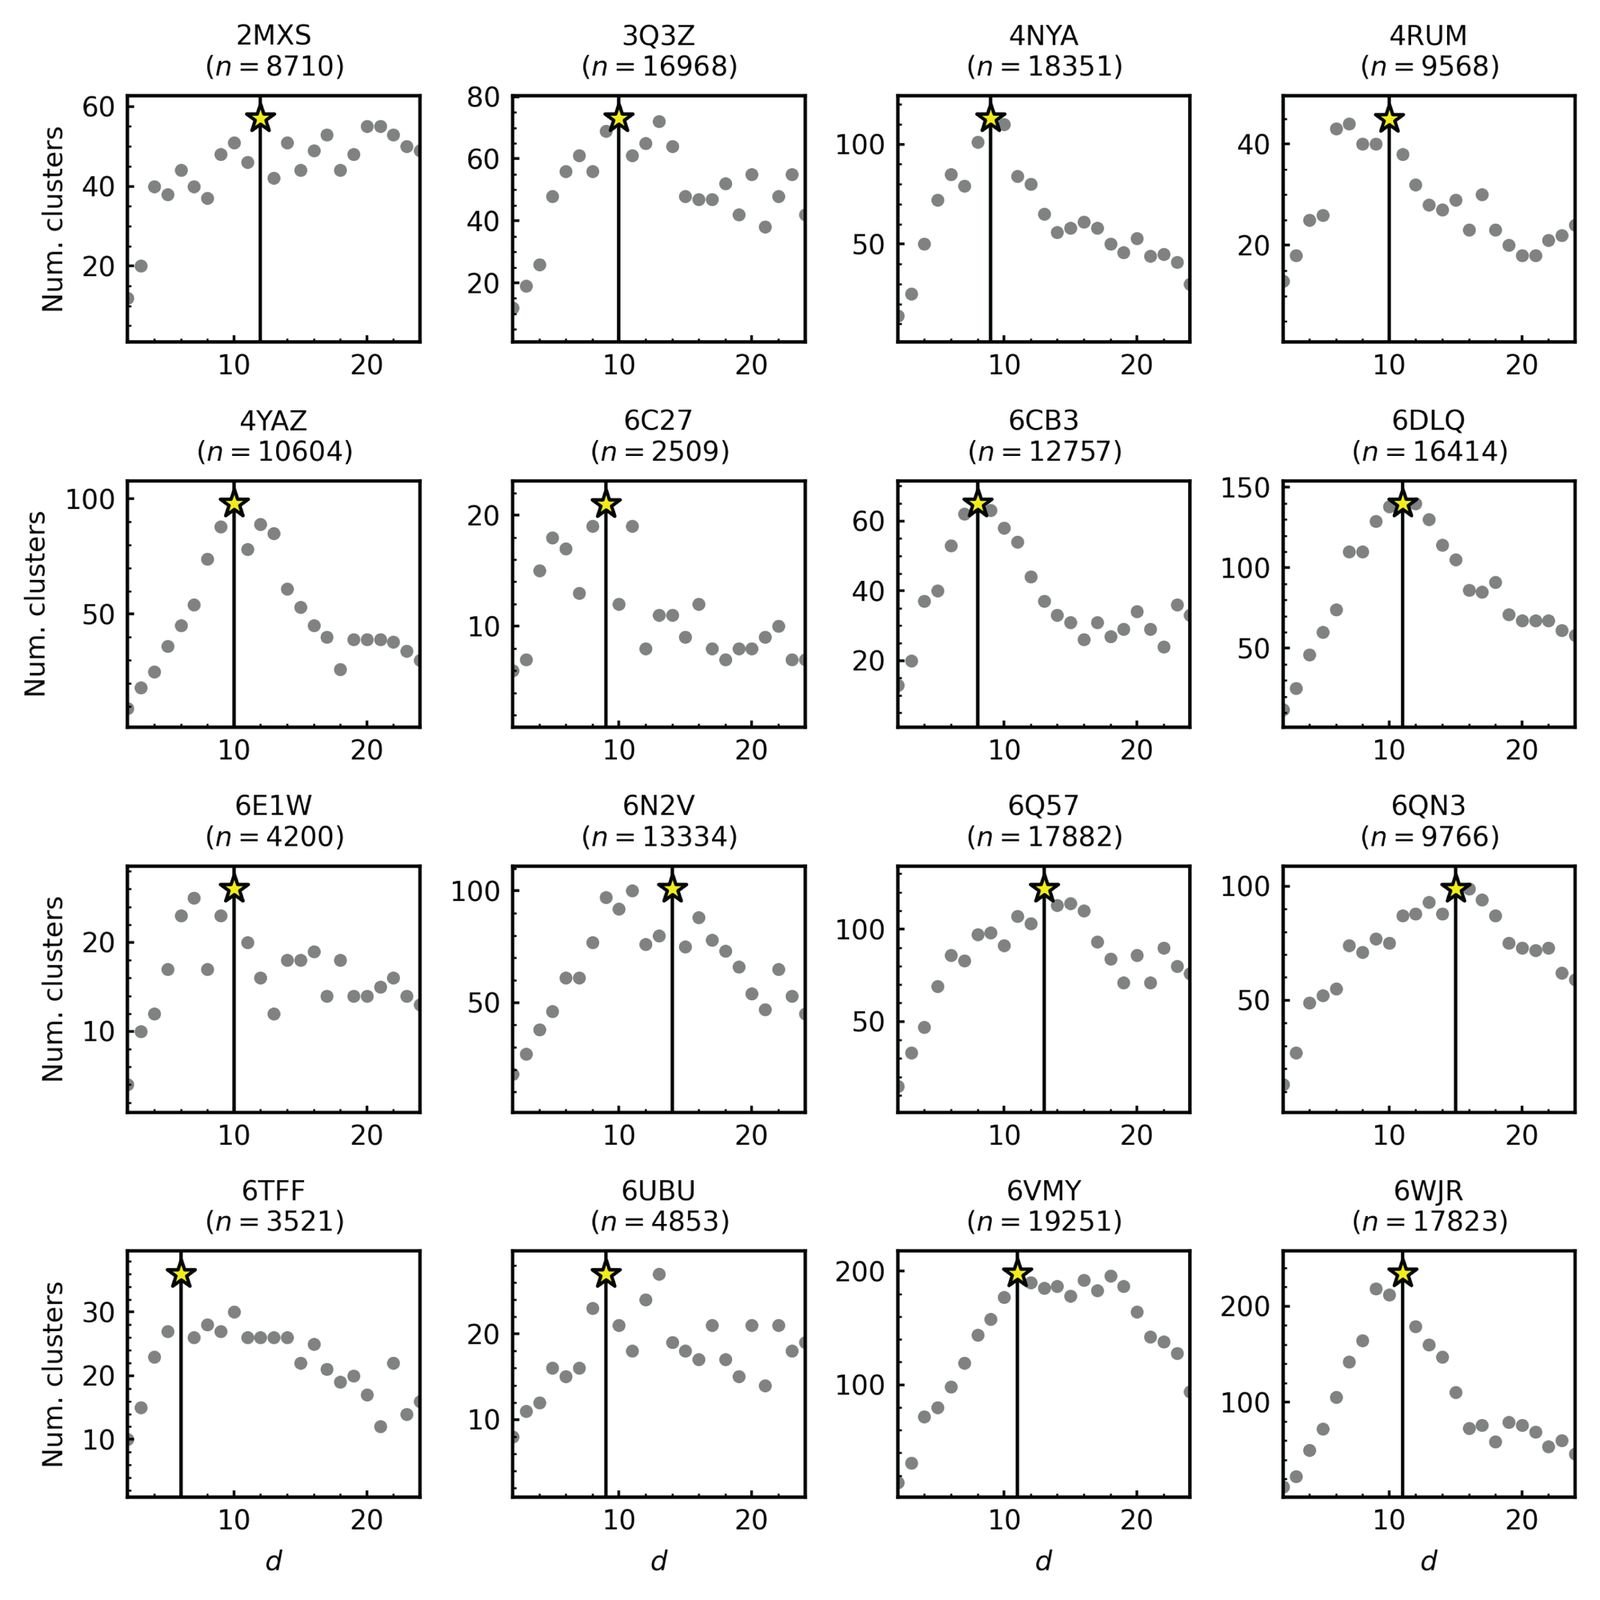
\includegraphics[
    width=\textwidth
    ]{figures/ch6_clusters_vs_d.jpg}
    \caption[Number of clusters vs d.]{{\bf Number of clusters vs d.} For each RNA, the G-vectors are projected onto $d$ components, and clustering is performed via the Advanced Density Peaks algorithm implemented in \texttt{dadapy}. The number of clusters, $N_c$ is recorded as a function of $d$. The star values and vertical line indicate the $d$ where $N_c$ is maximized; $n$ denotes the total number of models used in the calculation.}
    \label{ch6:fig:clusters_vs_d}%
\end{figure}

\begin{figure}
    \centering
    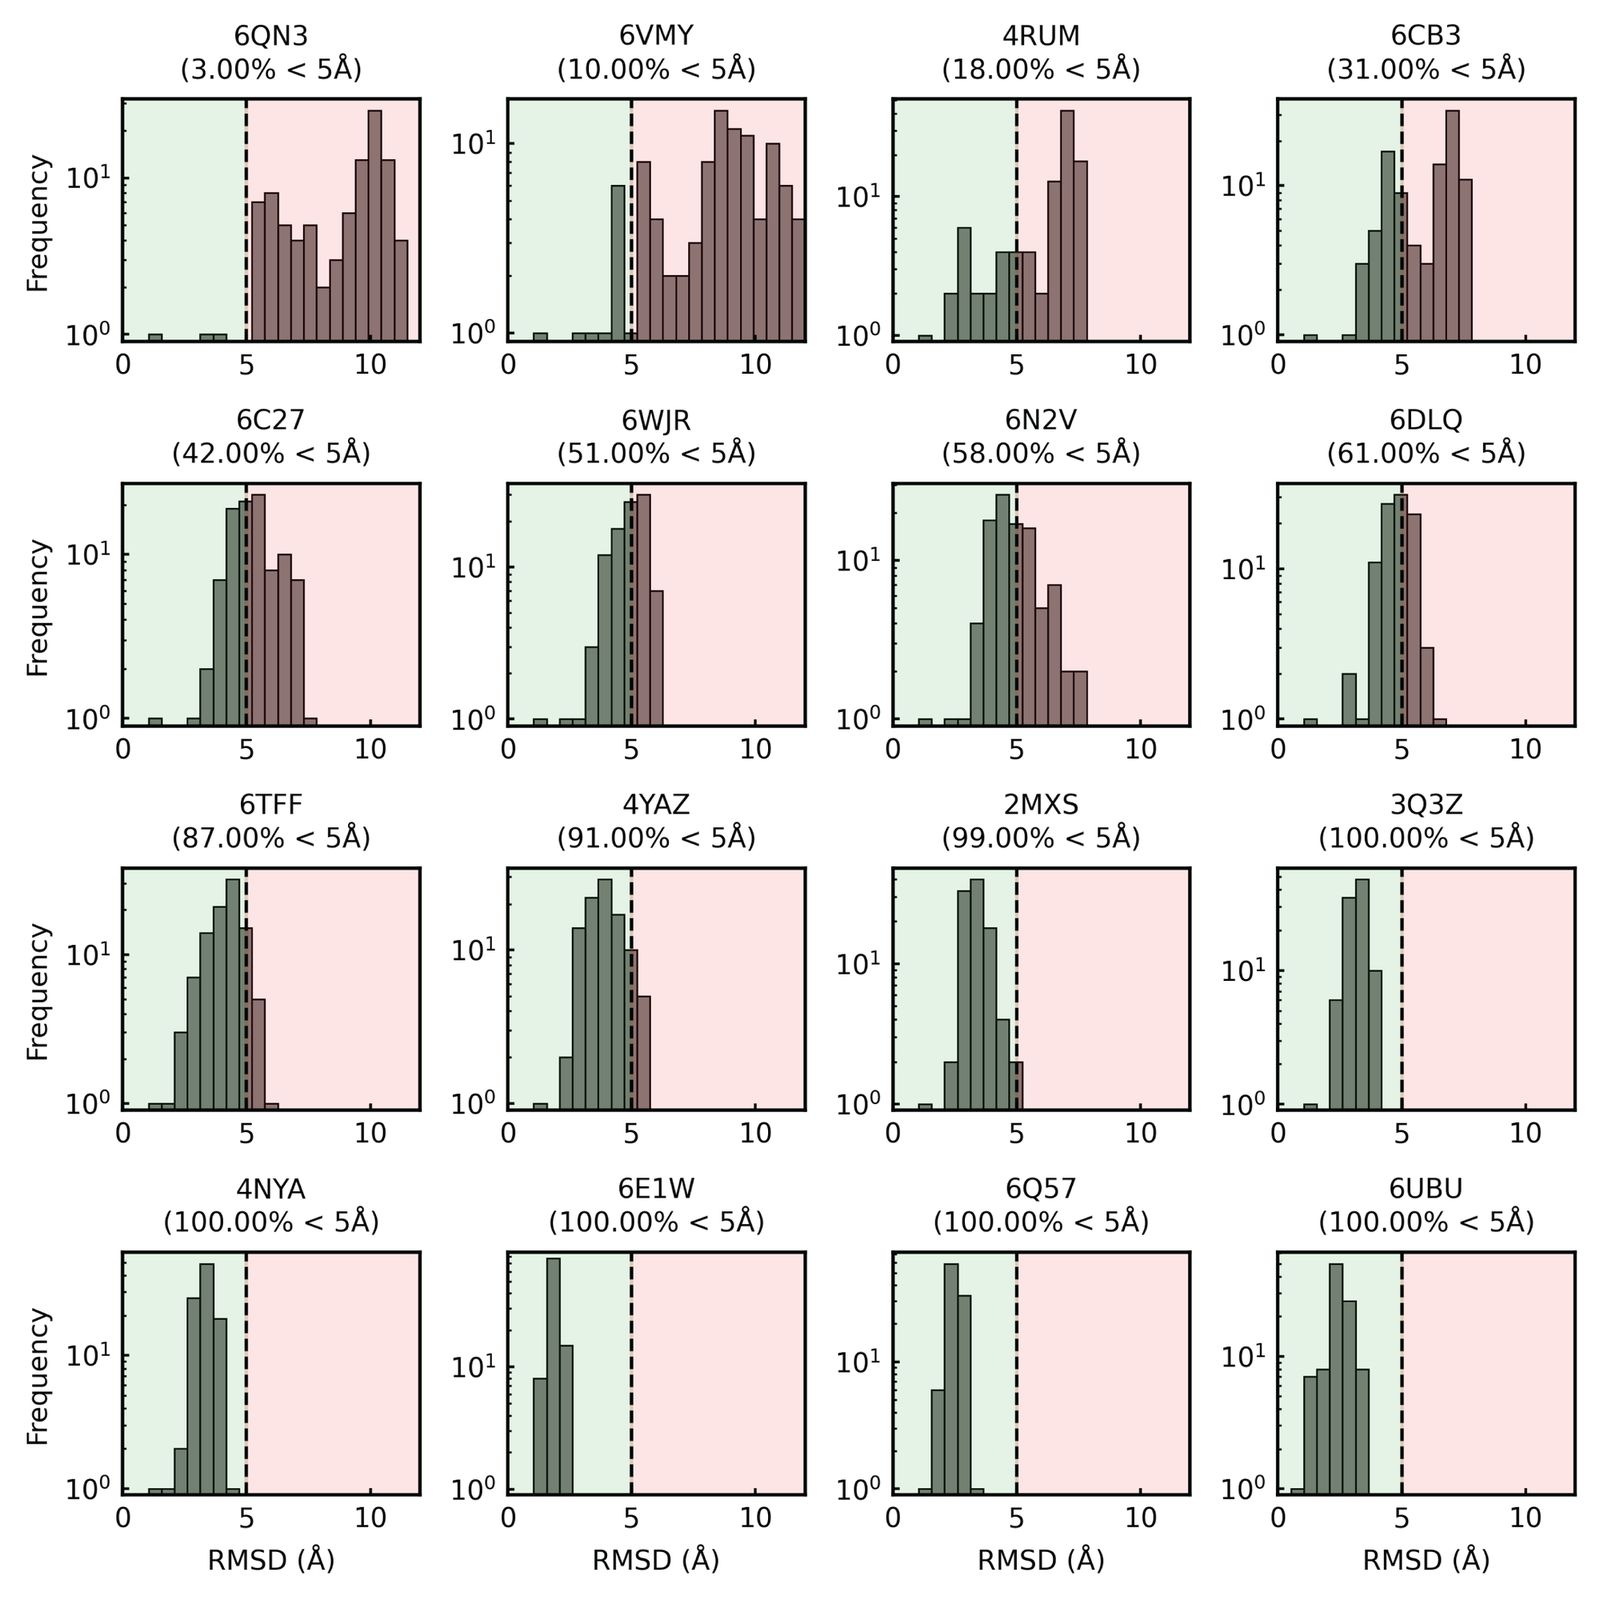
\includegraphics[
    width=\textwidth
    ]{figures/ch6_rmsd_reference.jpg}
    \caption[RMSD variation over a 100ns MD simulation launched from the reference conformation.]{{\bf RMSD variation over a 100ns MD simulation launched from the reference conformation.} The dashed line placed at $5${\AA} indicates the cutoff used to classify ERCs (RMSD$\leq5${\AA}) and decoys (RMSD $>5${\AA}) conformations. The proportion of ERCs is provided underneath the PDB accession code.}
    \label{ch6:fig:rmsd_reference}%
\end{figure}

\begin{figure}
    \centering
    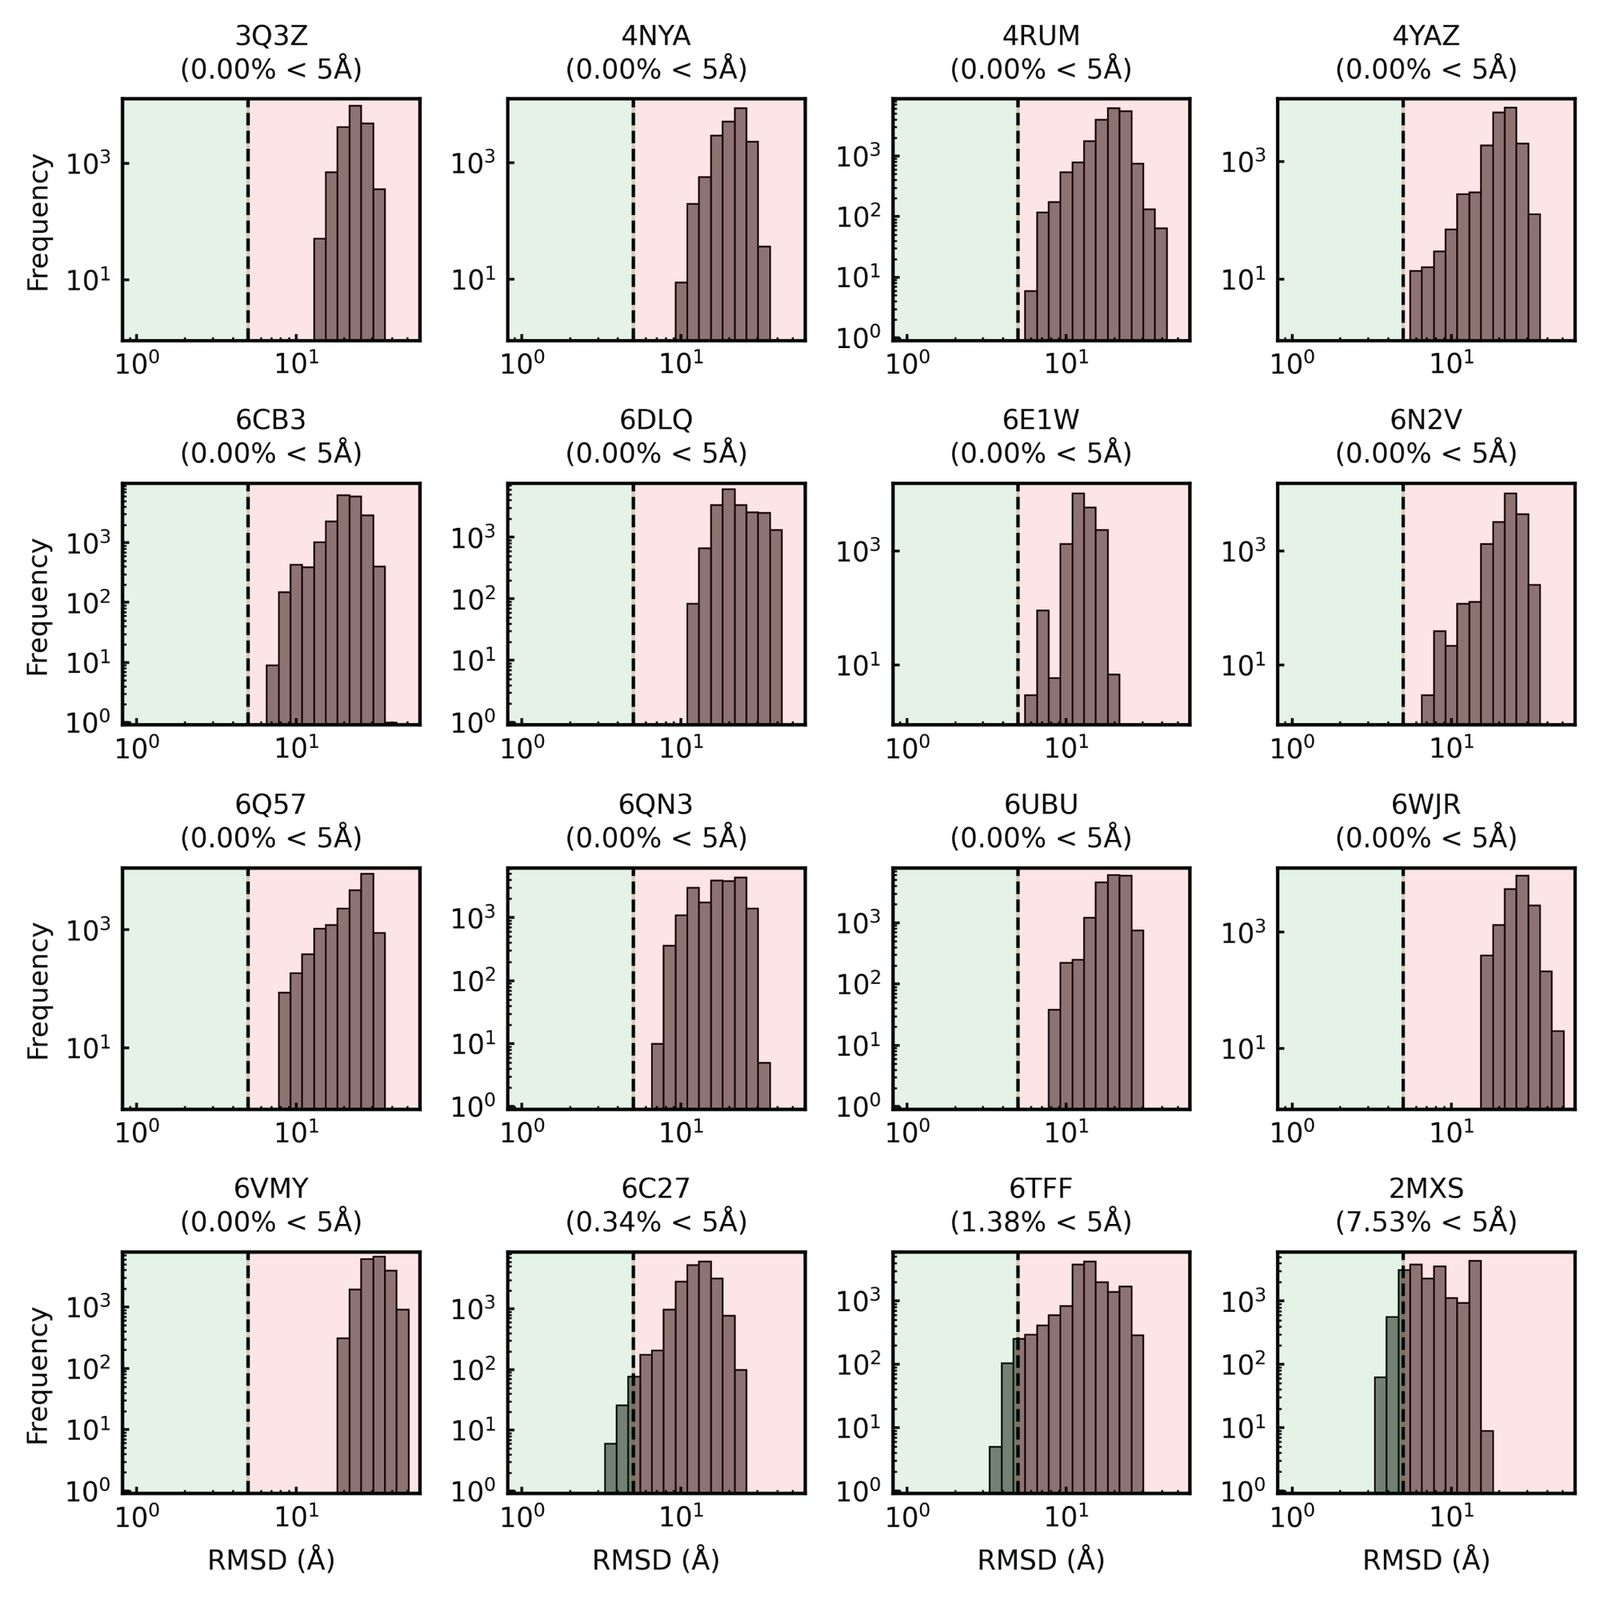
\includegraphics[
    width=\textwidth
    ]{figures/ch6_rmsd_decoys.jpg}
    \caption[RMSD distribution of conformations sampled by RNAnneal.]{{\bf RMSD distribution of conformations sampled by RNAnneal.} The dashed line placed at $5${\AA} indicates the cutoff used to classify ERCs (RMSD $\leq5${\AA}) and decoys (RMSD $>5${\AA}) conformations. The proportion of near-ERCs is provided underneath the PDB accession code.}
    \label{ch6:fig:rmsd_decoys}%
\end{figure}

\begin{figure}
    \centering
    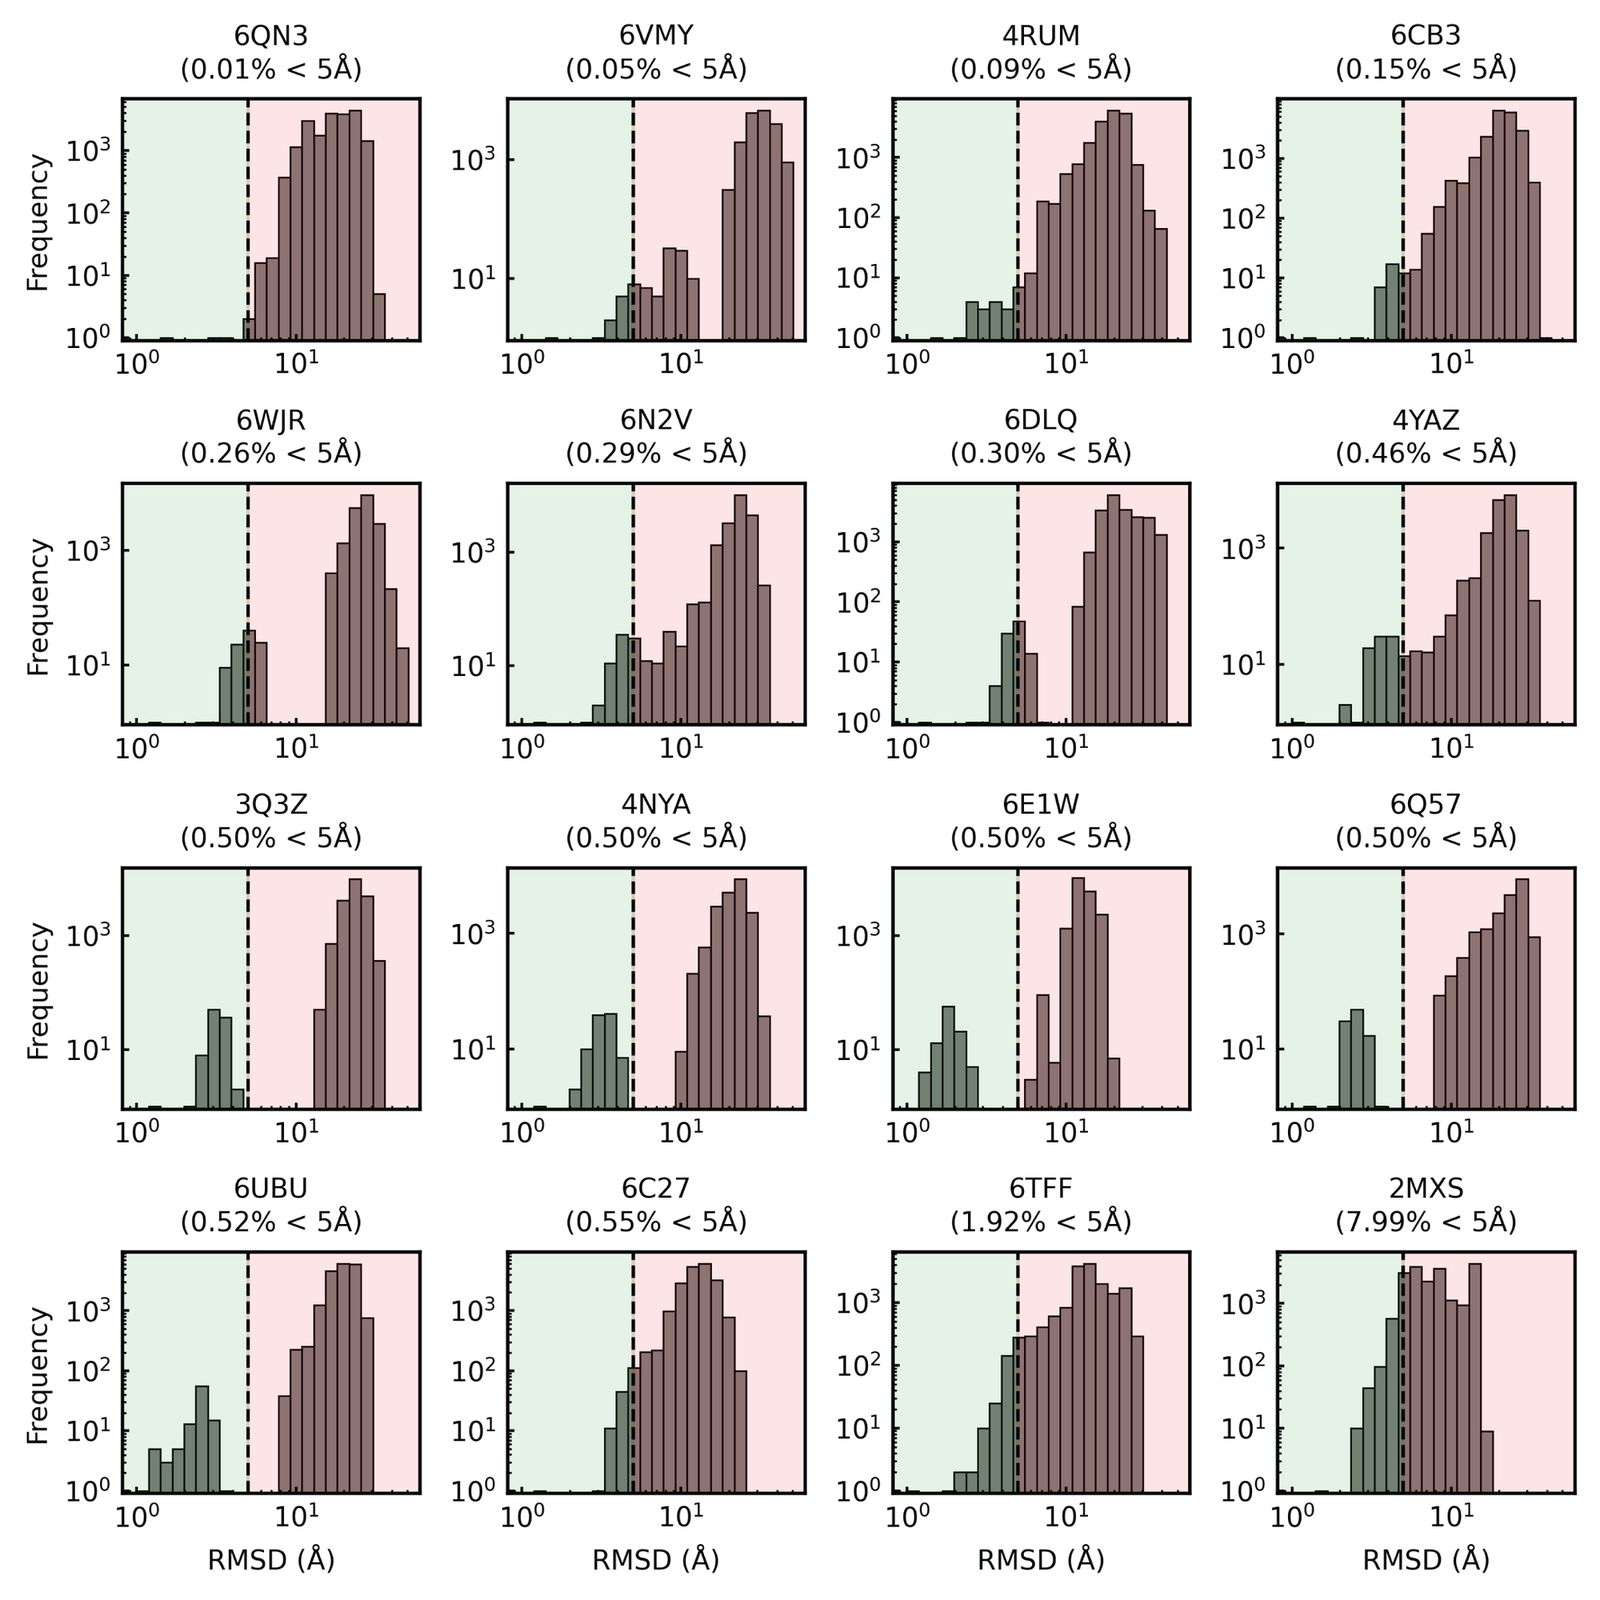
\includegraphics[
    width=\textwidth
    ]{figures/ch6_rmsd_combined.jpg}
    \caption[RMSD distribution of conformations for the classification task.]{{\bf RMSD distribution of conformations for the classification task.} The classification task merges structures sampled by RNAnneal with frames from simulations launched from the reference conformations (i.e., merges Fig. S\ref{ch6:fig:rmsd_reference} and S\ref{ch6:fig:rmsd_decoys}). The dashed line placed at $5${\AA} indicates the cutoff used to classify ERC (RMSD $\leq5${\AA}) and decoy (RMSD$>5${\AA}) conformations. The proportion of near-ERCs is provided underneath the PDB accession code.}
    \label{ch6:fig:rmsd_combined}%
\end{figure}

\begin{figure}
    \centering
    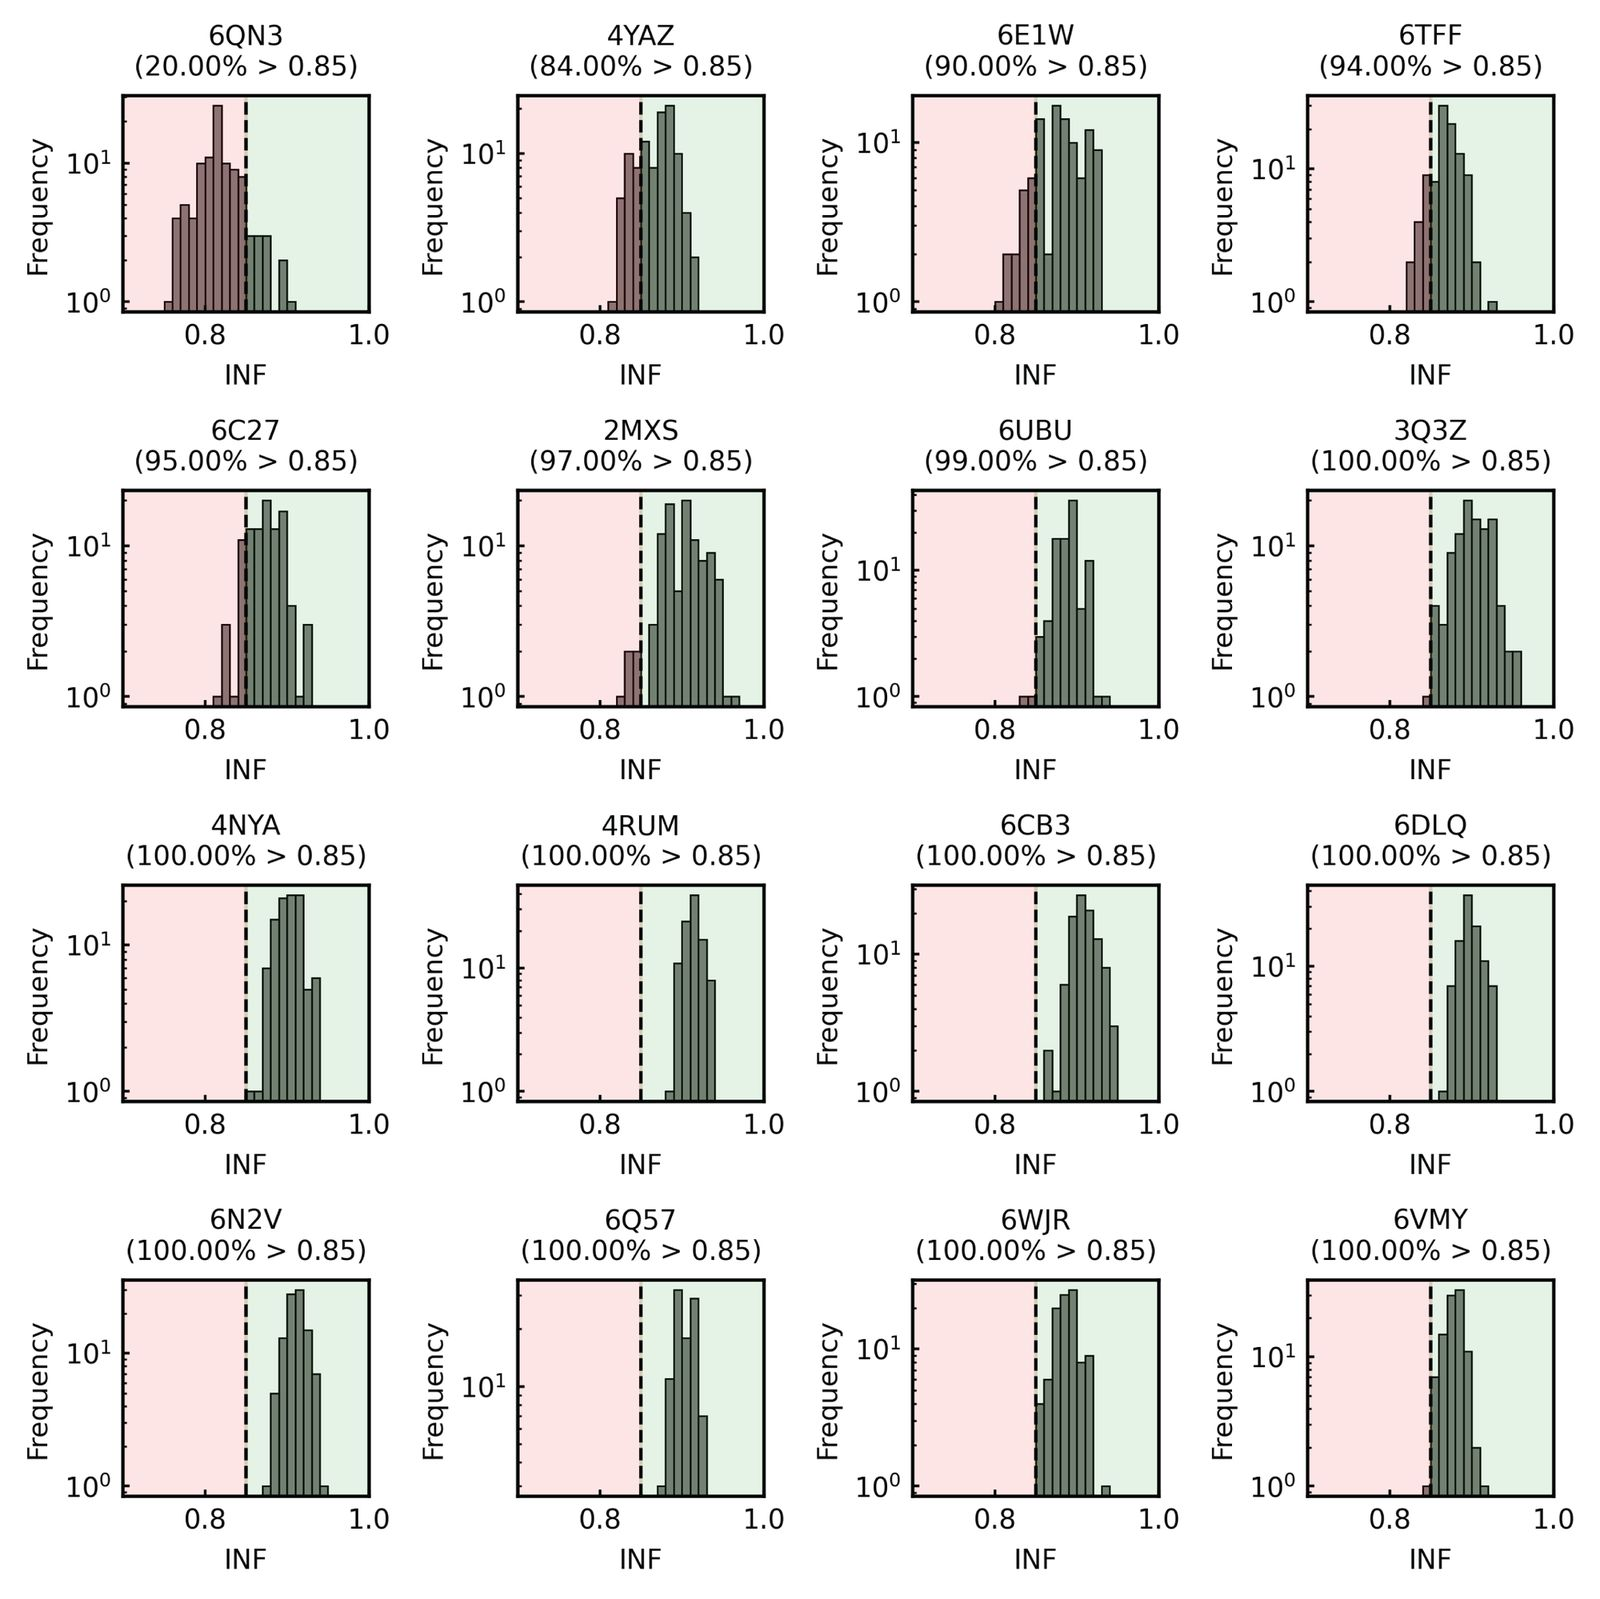
\includegraphics[
    width=\textwidth
    ]{figures/ch6_inf_reference.jpg}
    \caption[INF variation over a 100ns MD simulation launched from the reference conformation.]{{\bf INF variation over a 100ns MD simulation launched from the reference conformation.} The dashed line placed at $0.85$ indicates the cutoff used to classify ERC (INF$\geq$0.85) and decoy (INF$<$0.85) conformations. The proportion of near-ERCs is provided underneath the PDB accession code.}
    \label{ch6:fig:inf_reference}%
\end{figure}

\begin{figure}
    \centering
    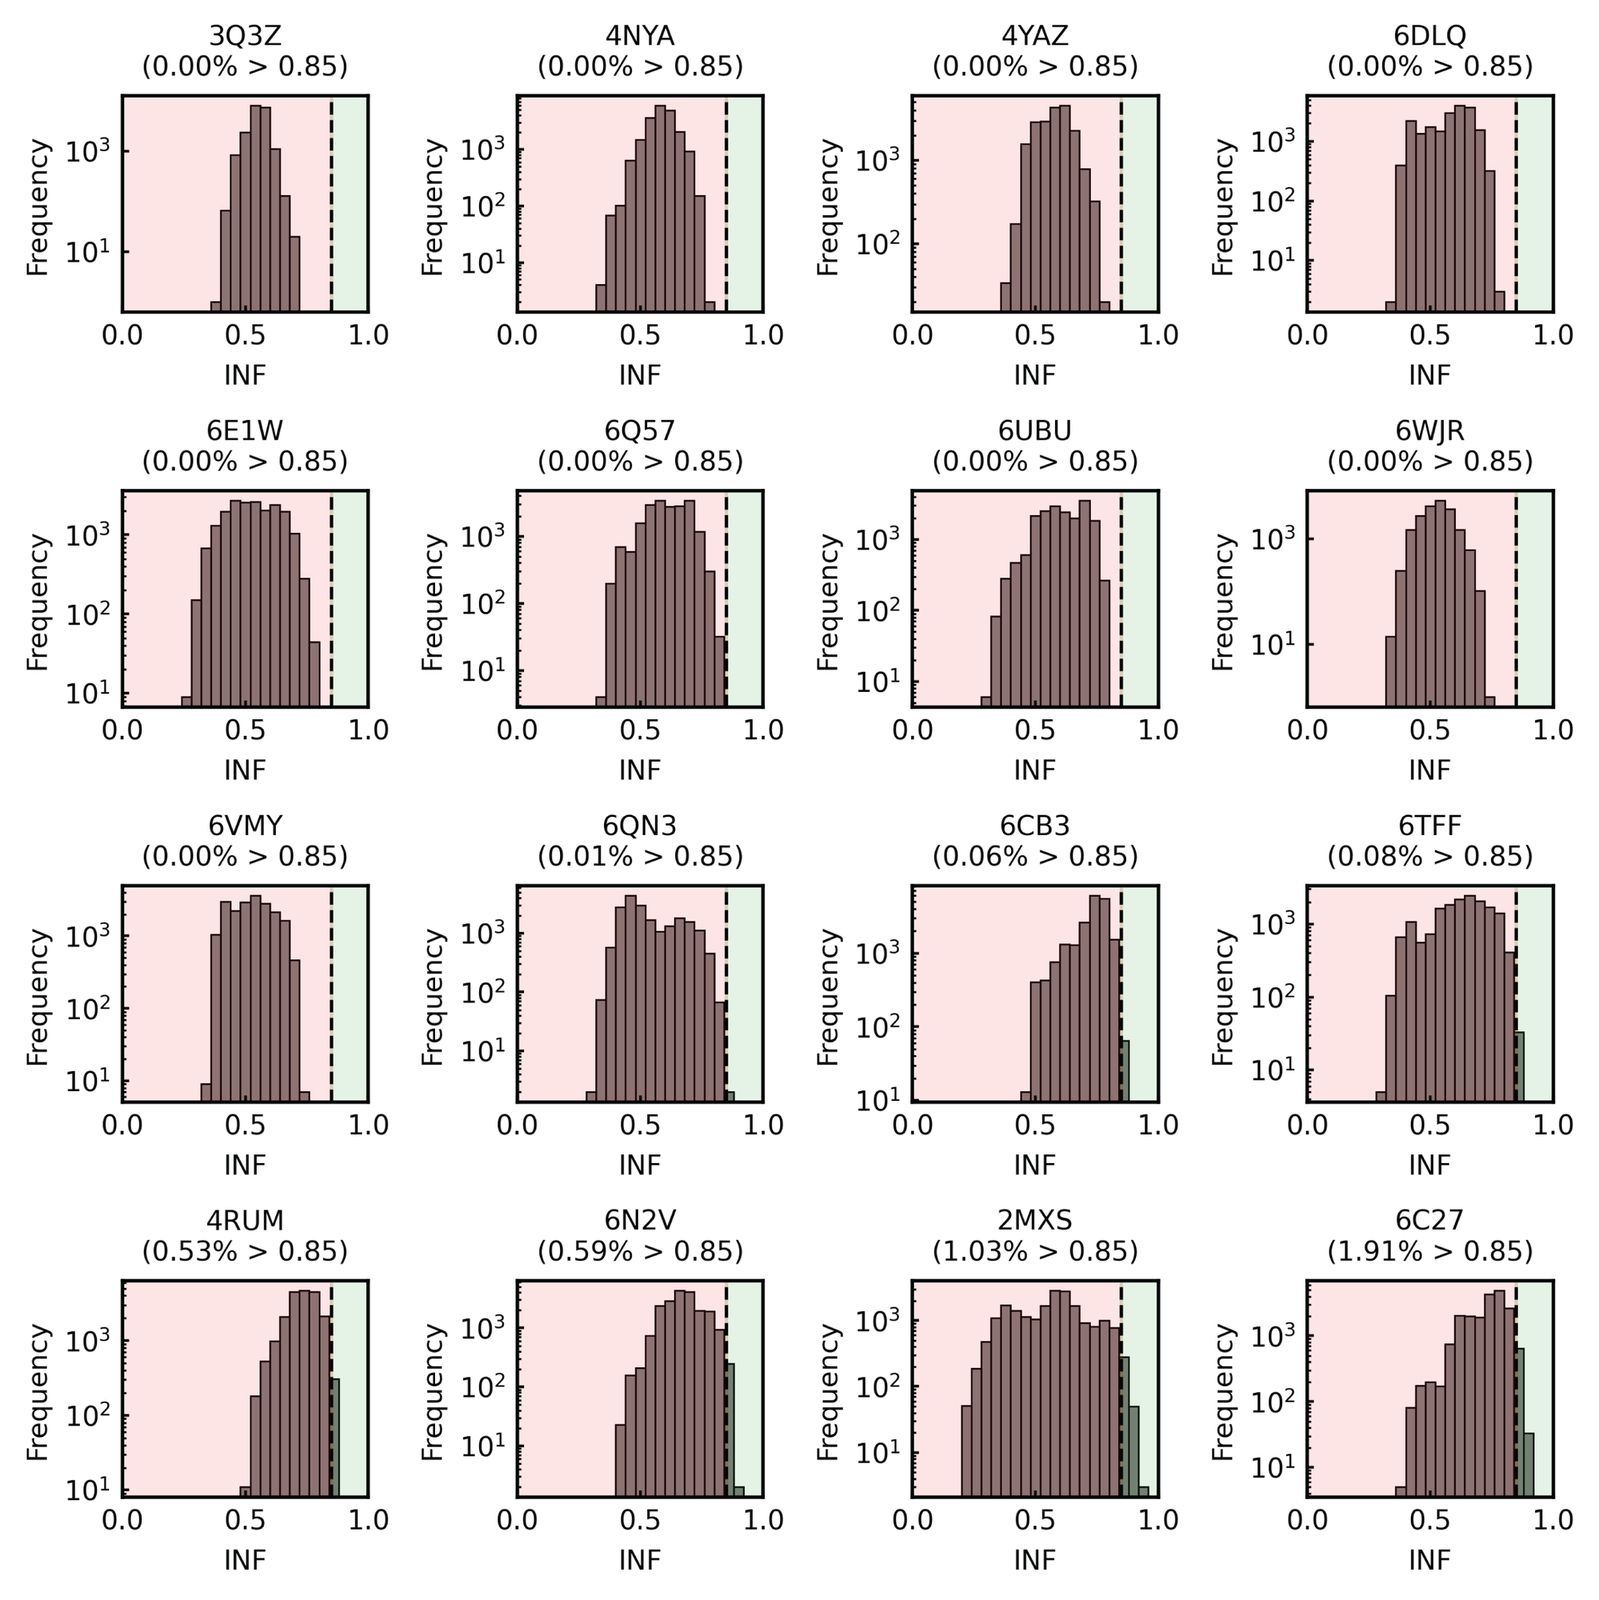
\includegraphics[
    width=\textwidth
    ]{figures/ch6_inf_decoys.jpg}
    \caption[INF distribution of conformations generated by RNAnneal.]{{\bf INF distribution of conformations generated by RNAnneal.} The dashed line placed at $0.85$ indicates the cutoff used to classify ERC (INF$\geq$0.85) and decoy (INF$<$0.85) conformations. The proportion of near-ERCs is provided underneath the PDB accession code.}
    \label{ch6:fig:inf_decoys}%
\end{figure}

\begin{figure}
    \centering
    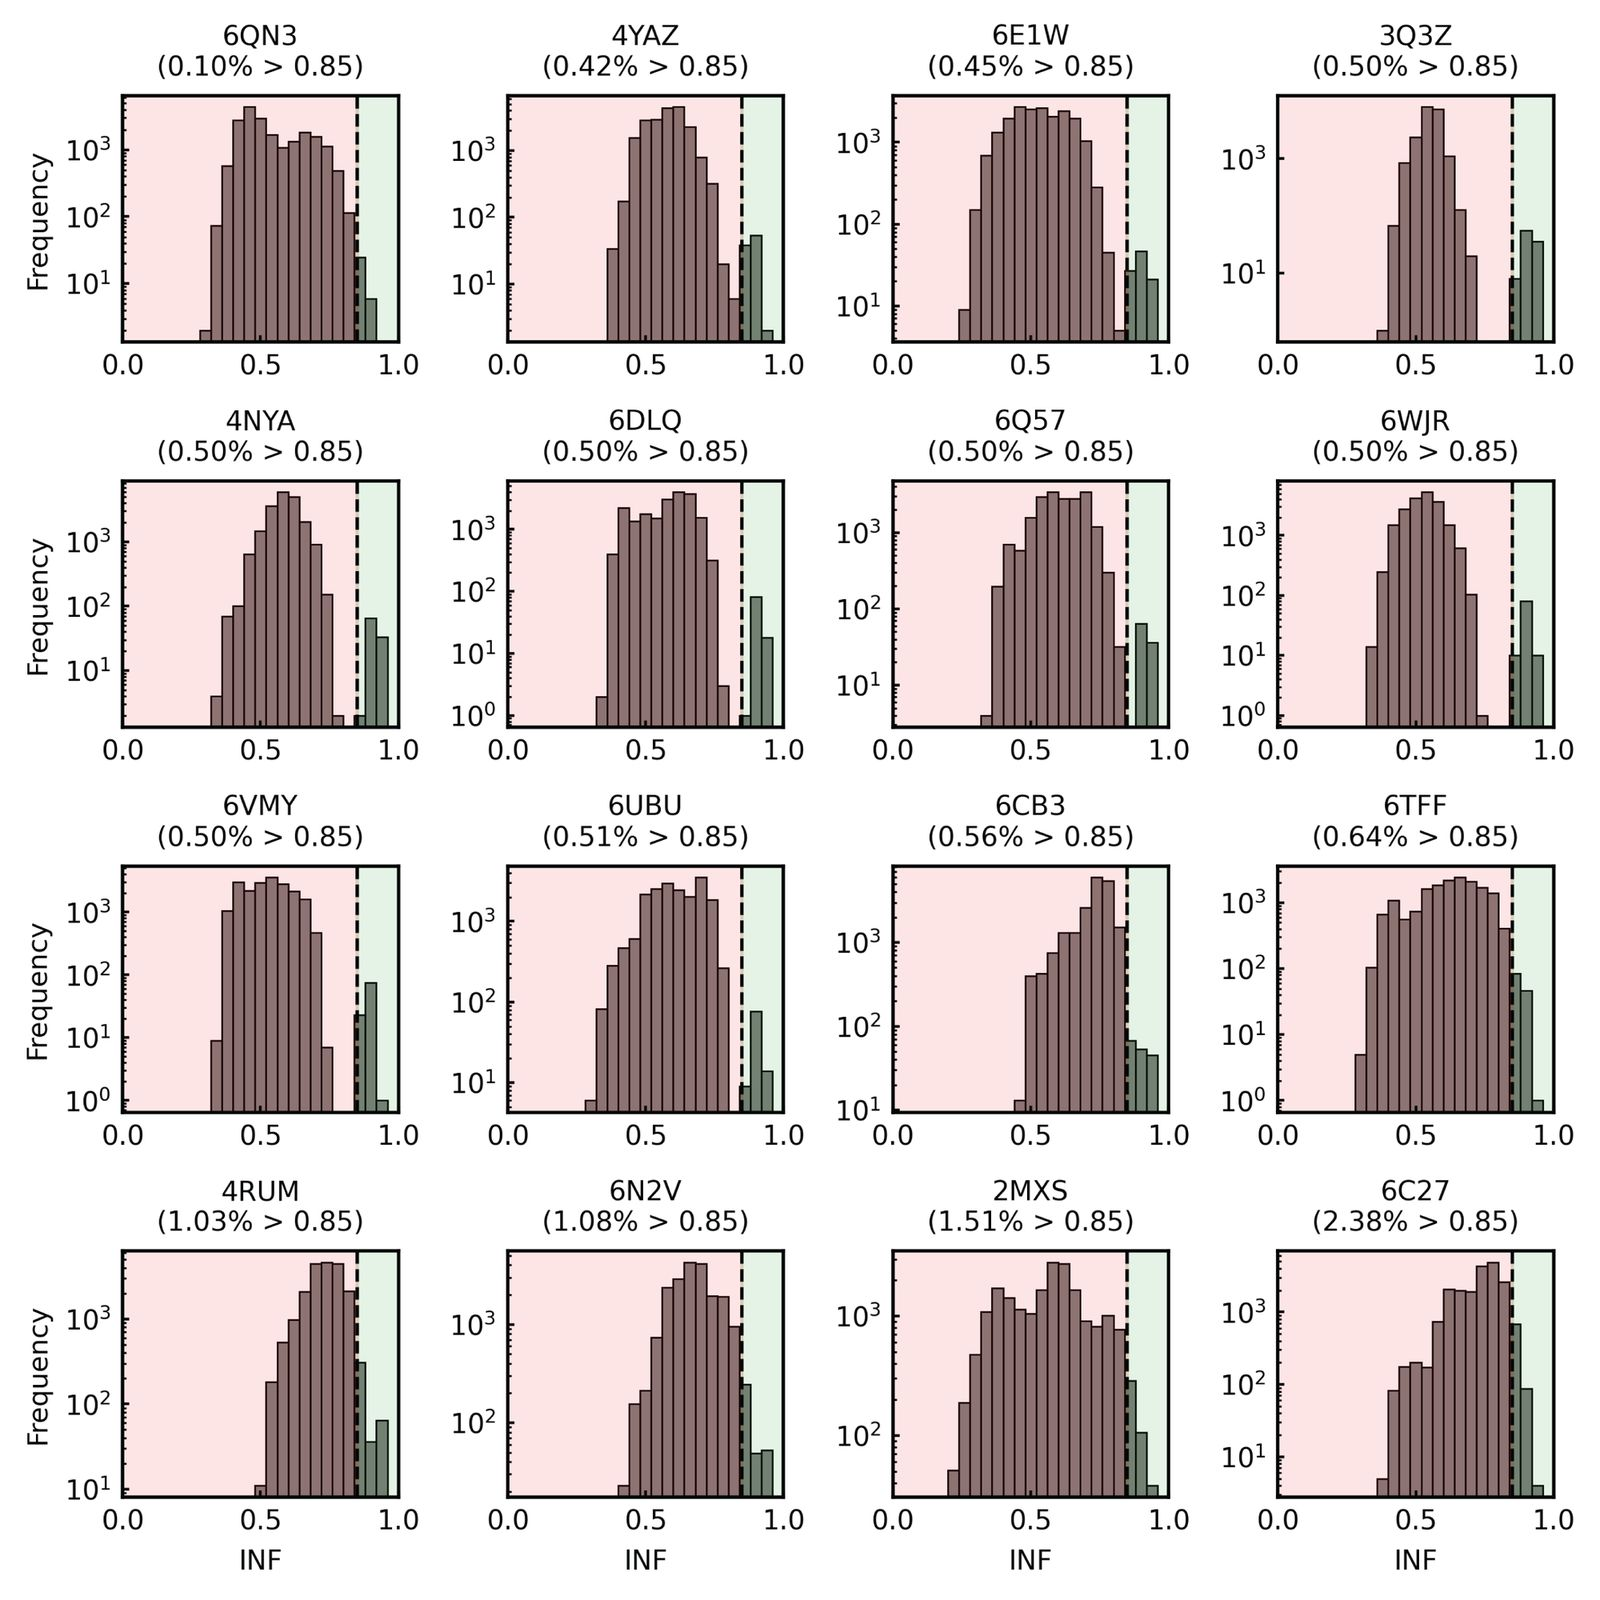
\includegraphics[
    width=\textwidth
    ]{figures/ch6_inf_combined.jpg}
    \caption[INF distribution of conformations for the classification task.]{{\bf INF distribution of conformations for the classification task.} The classification task merges structures sampled by RNAnneal with frames from simulations launched from the reference conformations (i.e., merges Fig. S\ref{ch6:fig:inf_reference} and S\ref{ch6:fig:inf_decoys}). The dashed line placed at $0.85$ indicates the cutoff used to classify ERC (INF$\geq$0.85) and decoy (INF$<$0.85) conformations. The proportion of near-ERCs is provided underneath the PDB accession code.}
    \label{ch6:fig:inf_combined}%
\end{figure}

\begin{figure}
    \centering
    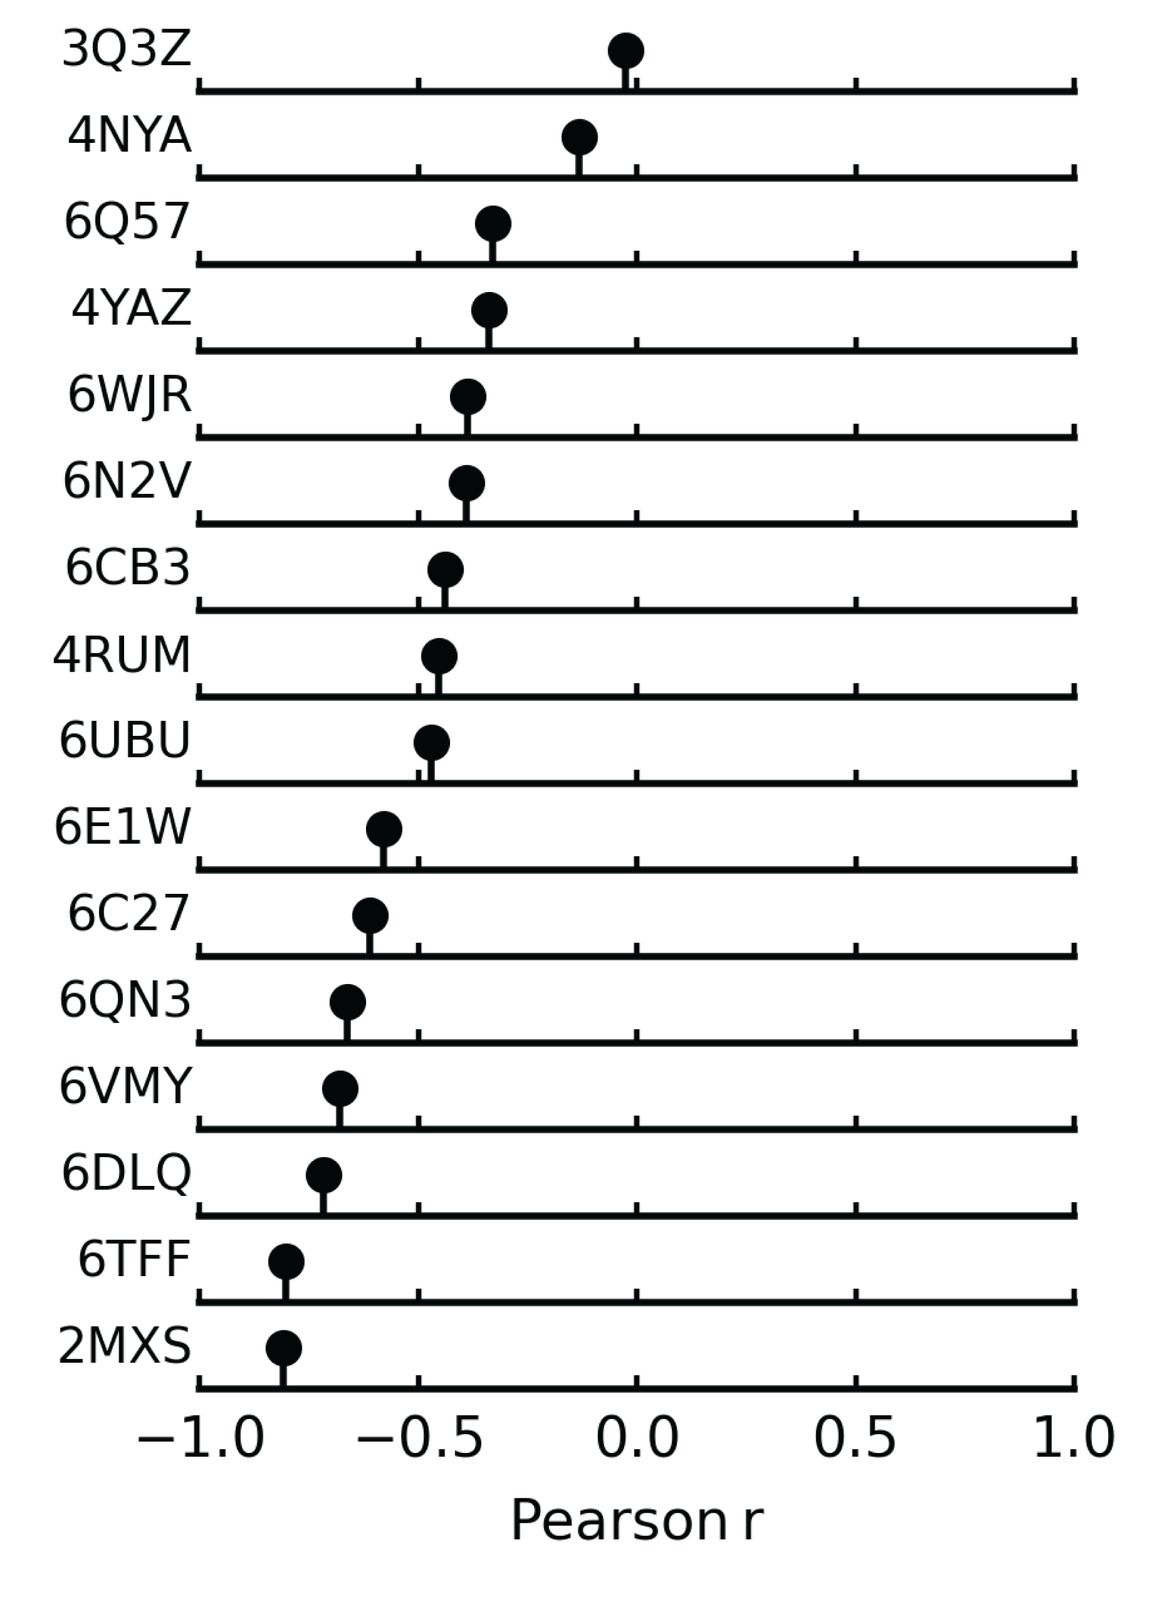
\includegraphics[
    width=0.4\textwidth
    ]{figures/ch6_correlation.jpg}
    \caption[Correlation between RMSD and INF for RNAnneal conformations.]{{\bf Correlation between RMSD and INF for RNAnneal conformations.}}
    \label{ch6:fig:correlation}%
\end{figure}

\begin{figure*}
    \centering
    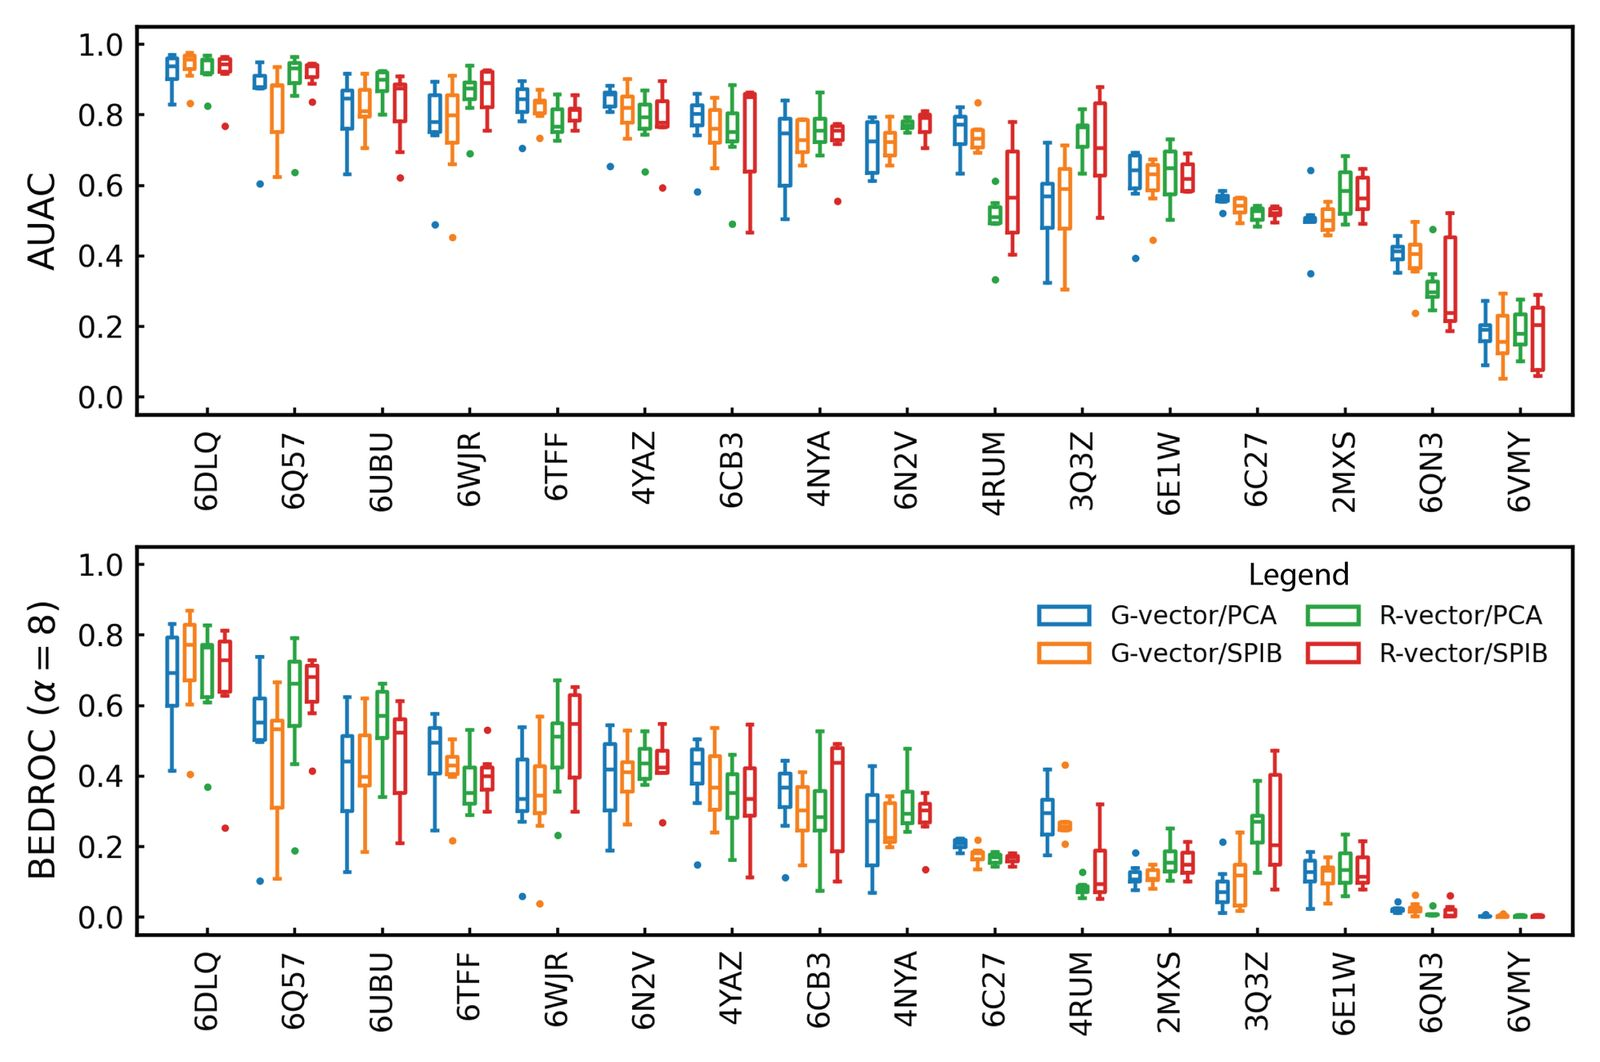
\includegraphics[
    width=0.9\textwidth
    ]{figures/ch6_auac-bedroc-by-feature.jpg}
    \caption[AUAC and BEDROC for each combination of training features.]{{\bf AUAC and BEDROC for each combination of training features.}}
    \label{ch6:fig:classification-by-feature}%
\end{figure*}

\begin{figure*}
    \centering
    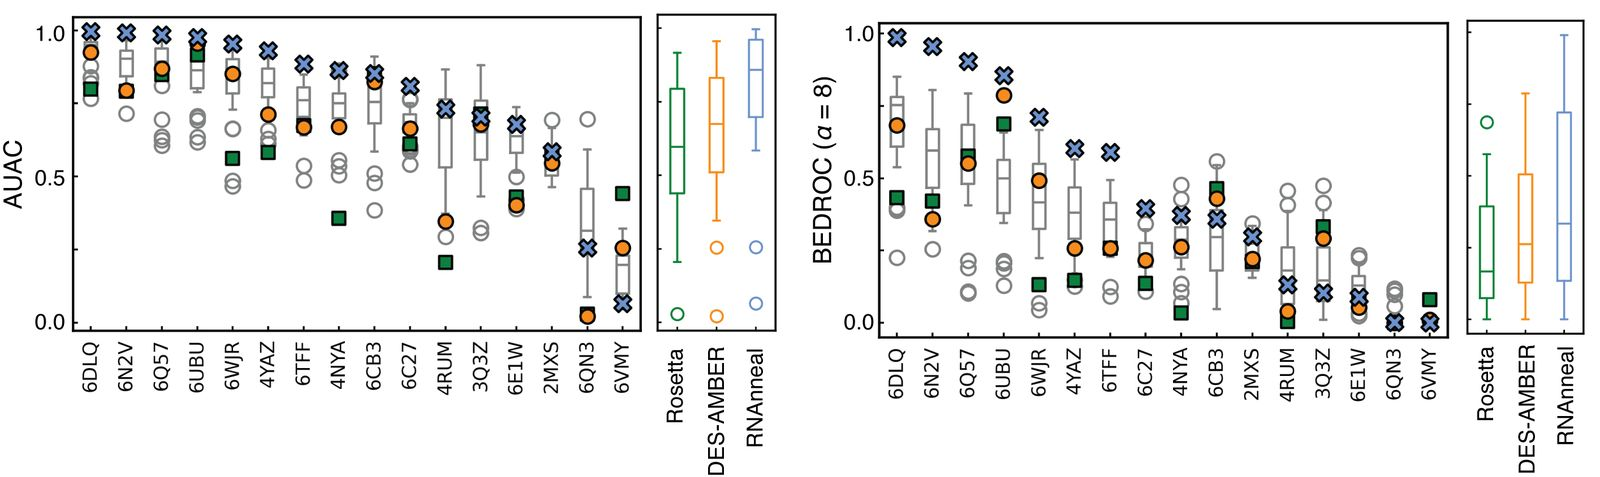
\includegraphics[
    width=\textwidth
    ]{figures/ch6_rmsd-enrichment.jpg}
    \caption[AUAC and BEDROC for RMSD classification criteria.]{{\bf AUAC and BEDROC for RMSD classification criteria.} Classification power of the Rosetta (blue), DES-AMBER (orange), and RNAnneal (blue) scores when ERCs are defined as conformations $<5${\AA} in RMSD from the reference conformation. The gray boxplots show the distribution of AUAC and BEDROC values for each model in the TM ensemble.}
    \label{ch6:fig:rmsd-enrichment}%
\end{figure*}

\begin{figure}
    \centering
    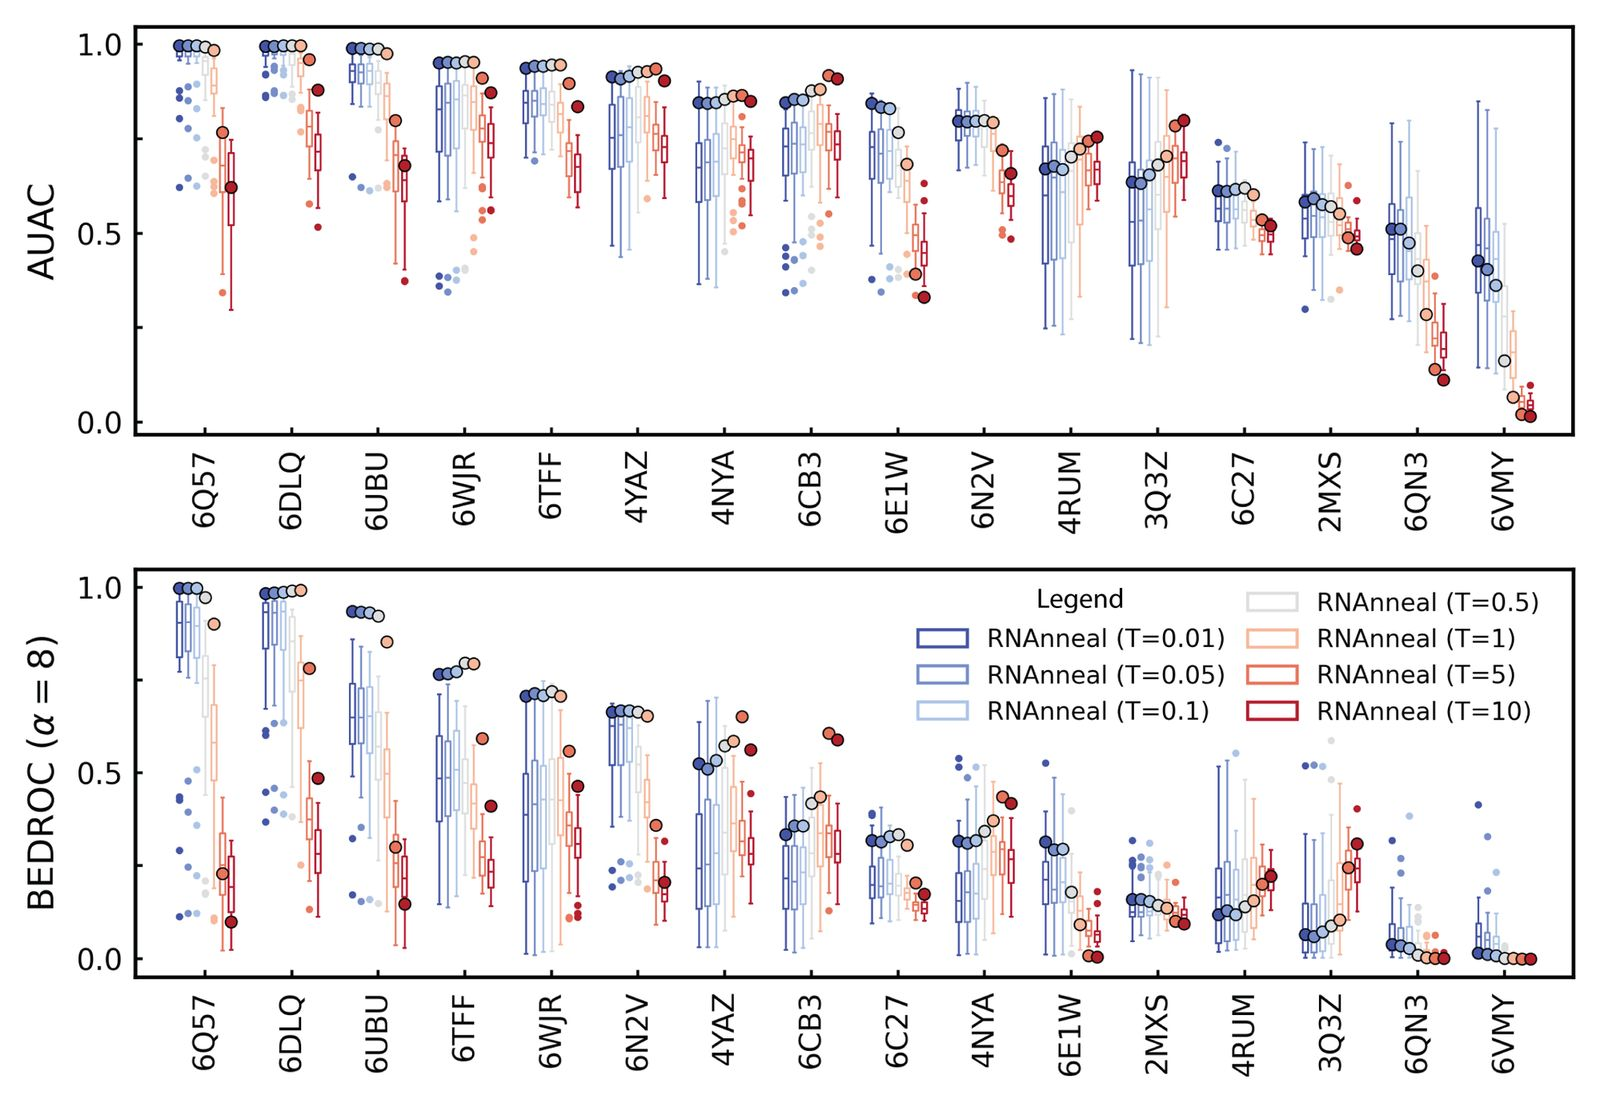
\includegraphics[
    width=0.9\textwidth
    ]{figures/ch6_enrichment-temperature-dependence.jpg}
    \caption[Variation in AUAC and BEDROC with scoring temperature.]{{\bf Variation in AUAC and BEDROC with scoring temperature.}}
    \label{ch6:fig:model-temp-dependence}%
\end{figure}

% \begin{figure*}
%     \centering
%     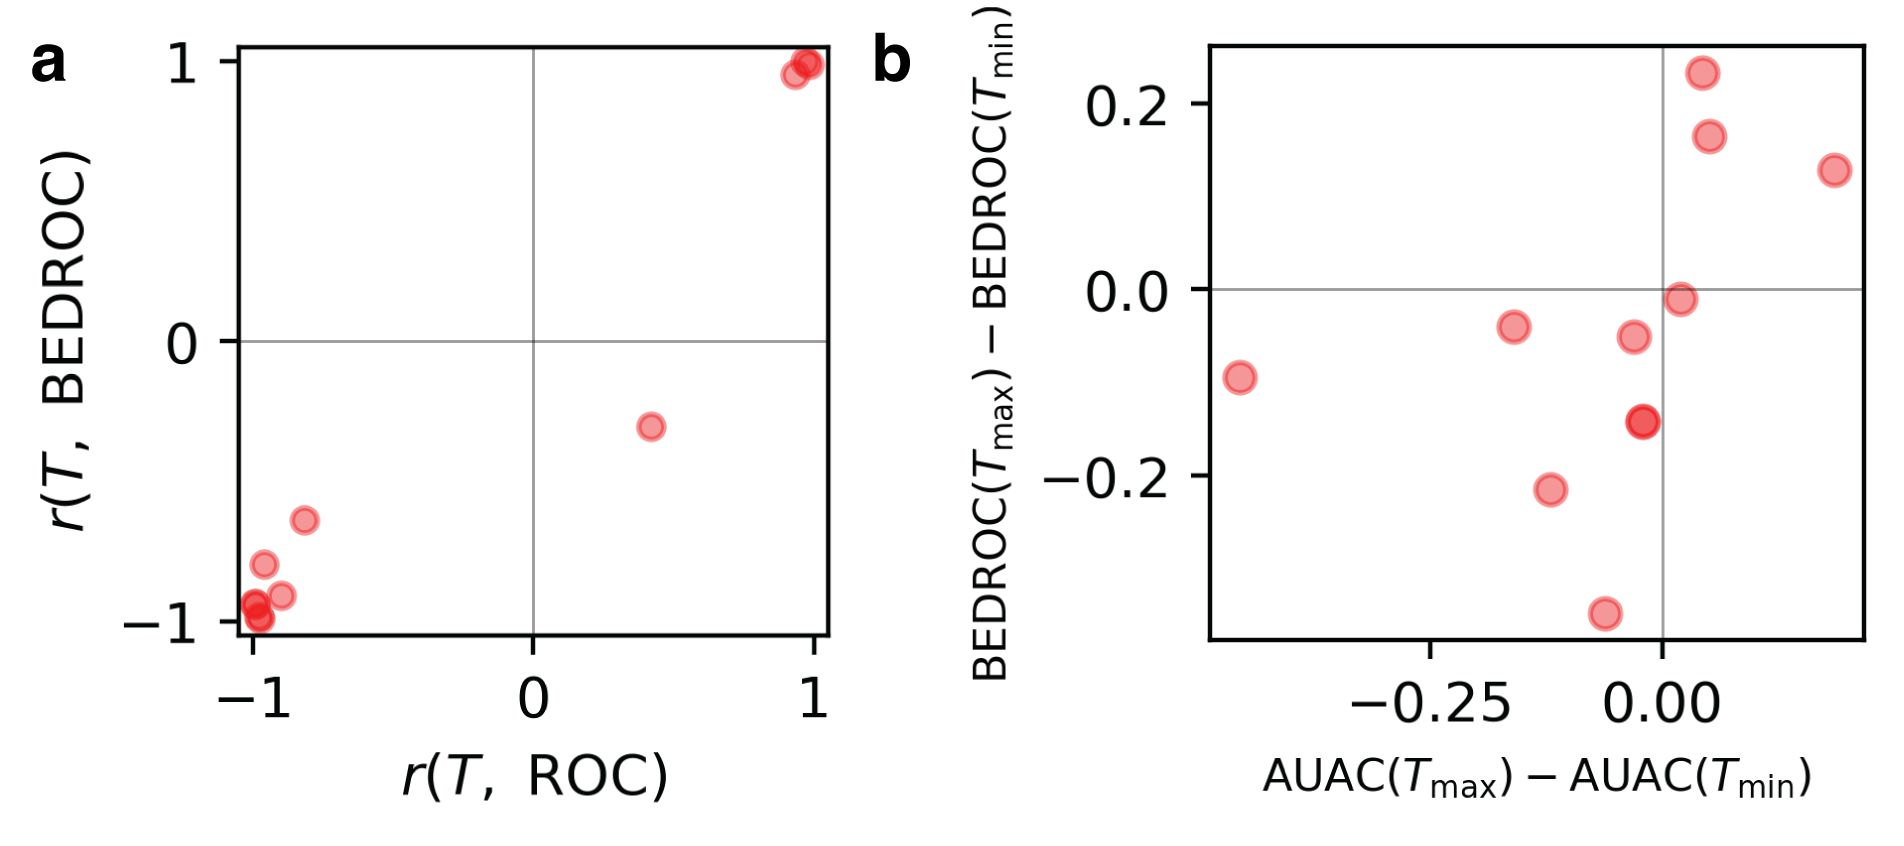
\includegraphics[
%     width=0.75\textwidth
%     ]{figures/ch6_auac-bedroc-temperature-analysis.jpg}
%     \caption[The effect of model temperature on AUAC and BEDROC]{{\bf The effect of model temperature on AUAC and BEDROC} (a) The correlation between AUAC and BEDROC values and model temperature $T \in \{0.1, 0.5, 1.0, 1.5, 2.0, 2.5\}$ is reported. For all but three RNAs increasing temperature linearly decreases AUAC and BEDROC. (b) The difference in AUAC and BEDROC at the minimum and maximum model temperature is reported. The AUAC and BEDROC value generally decreases as the temperature is raised.}
%     \label{ch6:fig:model-temperature}%
% \end{figure*}

\begin{figure*}
    \centering
    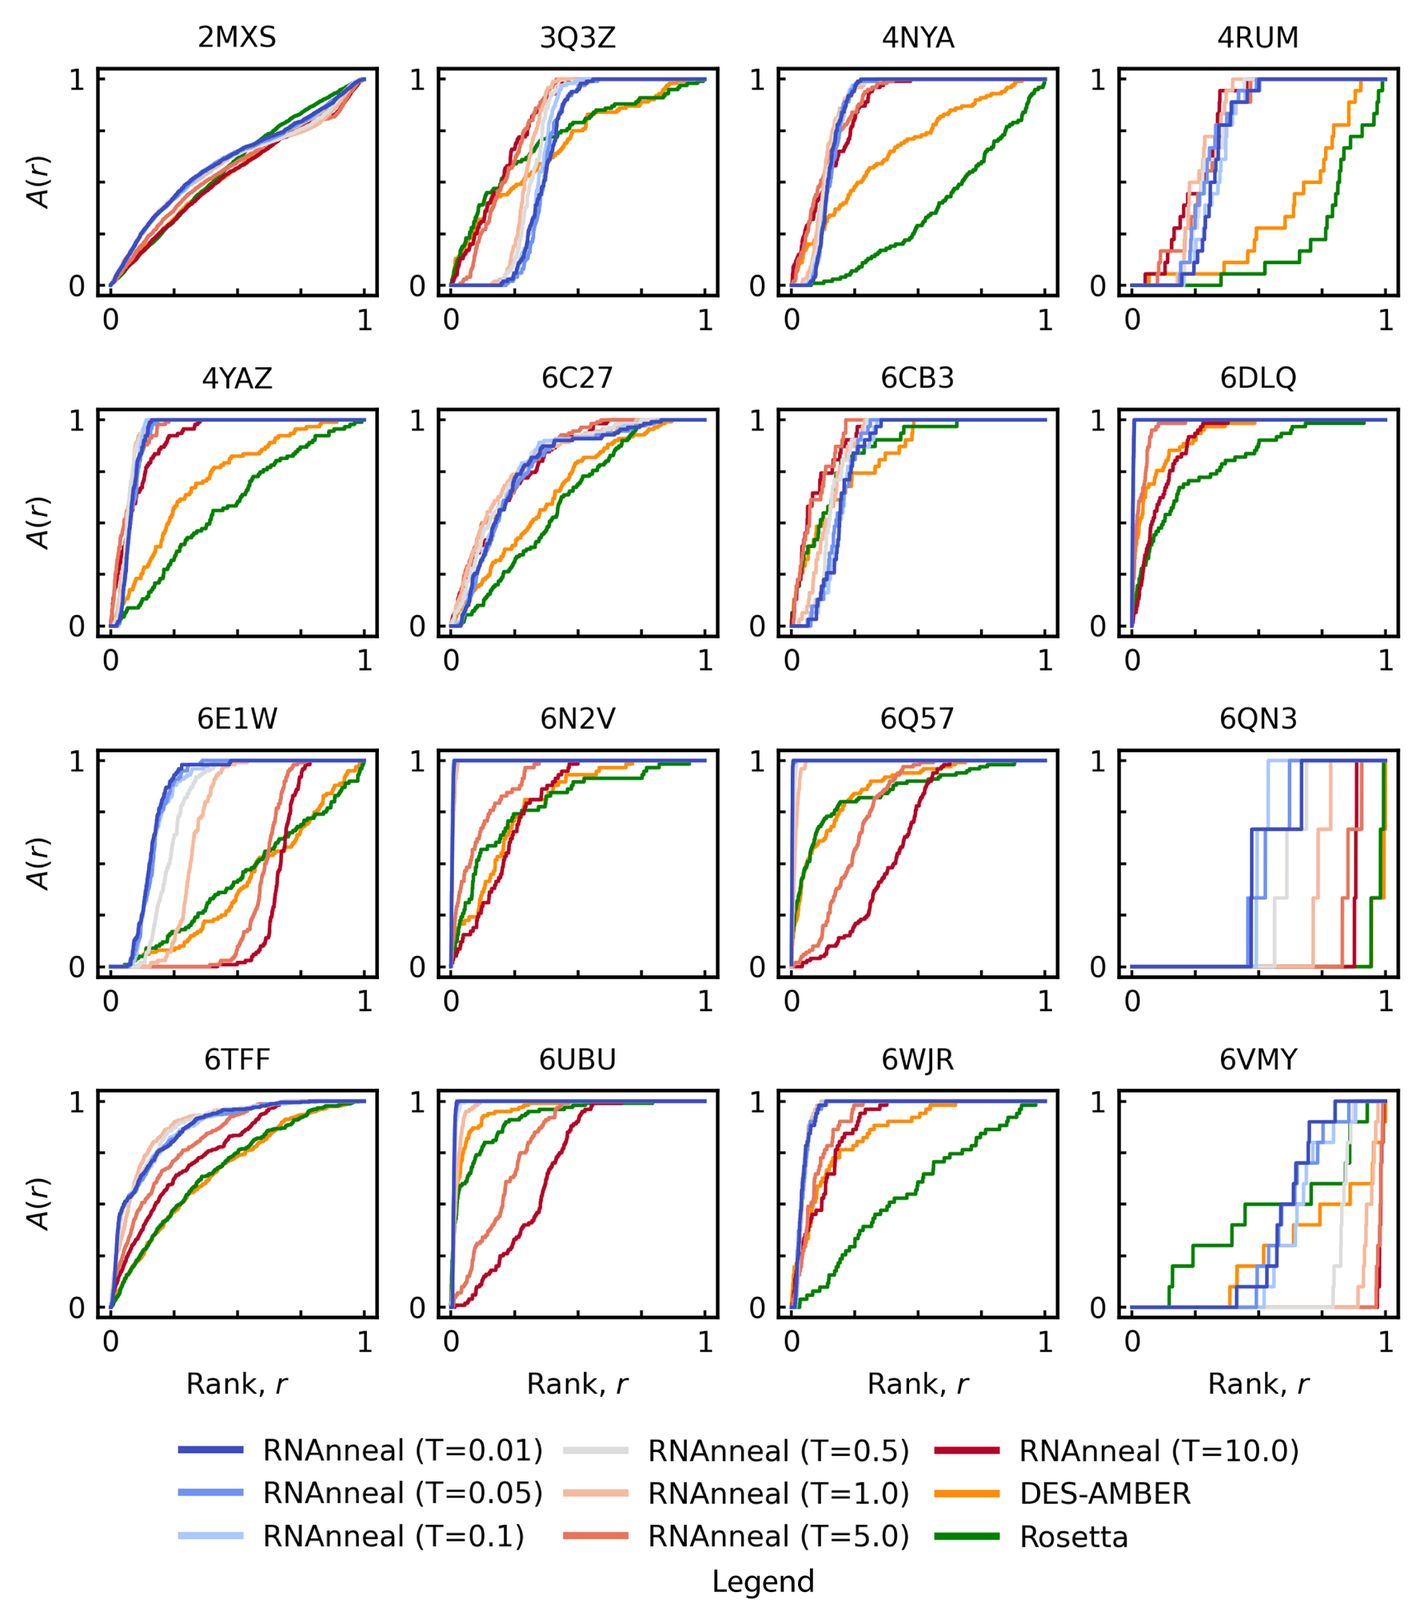
\includegraphics[
    width=\textwidth
    ]{figures/ch6_accum_curves_inf.jpg}
    \caption[Accumulation Curves.]{{\bf Accumulation Curves.} Accumulation curves, $A(r)$ are reported for each riboswitch, identified by the PDB entry of the reference conformation.}
    \label{ch6:fig:acc-curves}%
\end{figure*}

\begin{figure*}
    \centering
    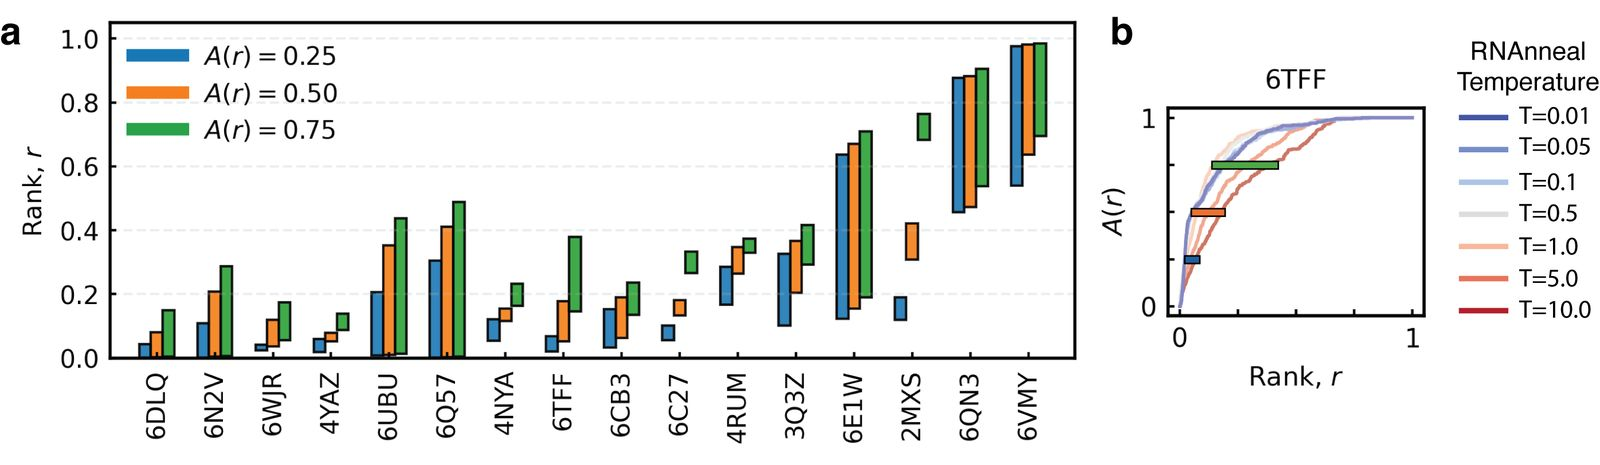
\includegraphics[
    width=\textwidth
    ]{figures/ch6_accumulation-curve-summary.jpg}
    \caption[Summary of Accumulation Curves]{{\bf Summary of Accumulation Curves} \textbf{a.} The set of accumulation curves for each riboswitch PDB is shown with the range of rank, $r$, for which $A(r)=0.25$, $A(r)=0.50$, and $A(r)=0.75$. \textbf{b.} The range indicated by the bars shows the variation of $r$ with temperature at fixed values of $A(r)=0.25$, $A(r)=0.50$, and $A(r)=0.75$. The accumulation curve for the NAD$^{+}$ riboswitch (6E1W~\cite{Numata2019}) is shown as an example (see Fig. S\ref{ch6:fig:acc-curves} for all riboswitches).   }
    \label{ch6:fig:acc-curve-summary}%
\end{figure*}

\begin{figure*}
    \centering
    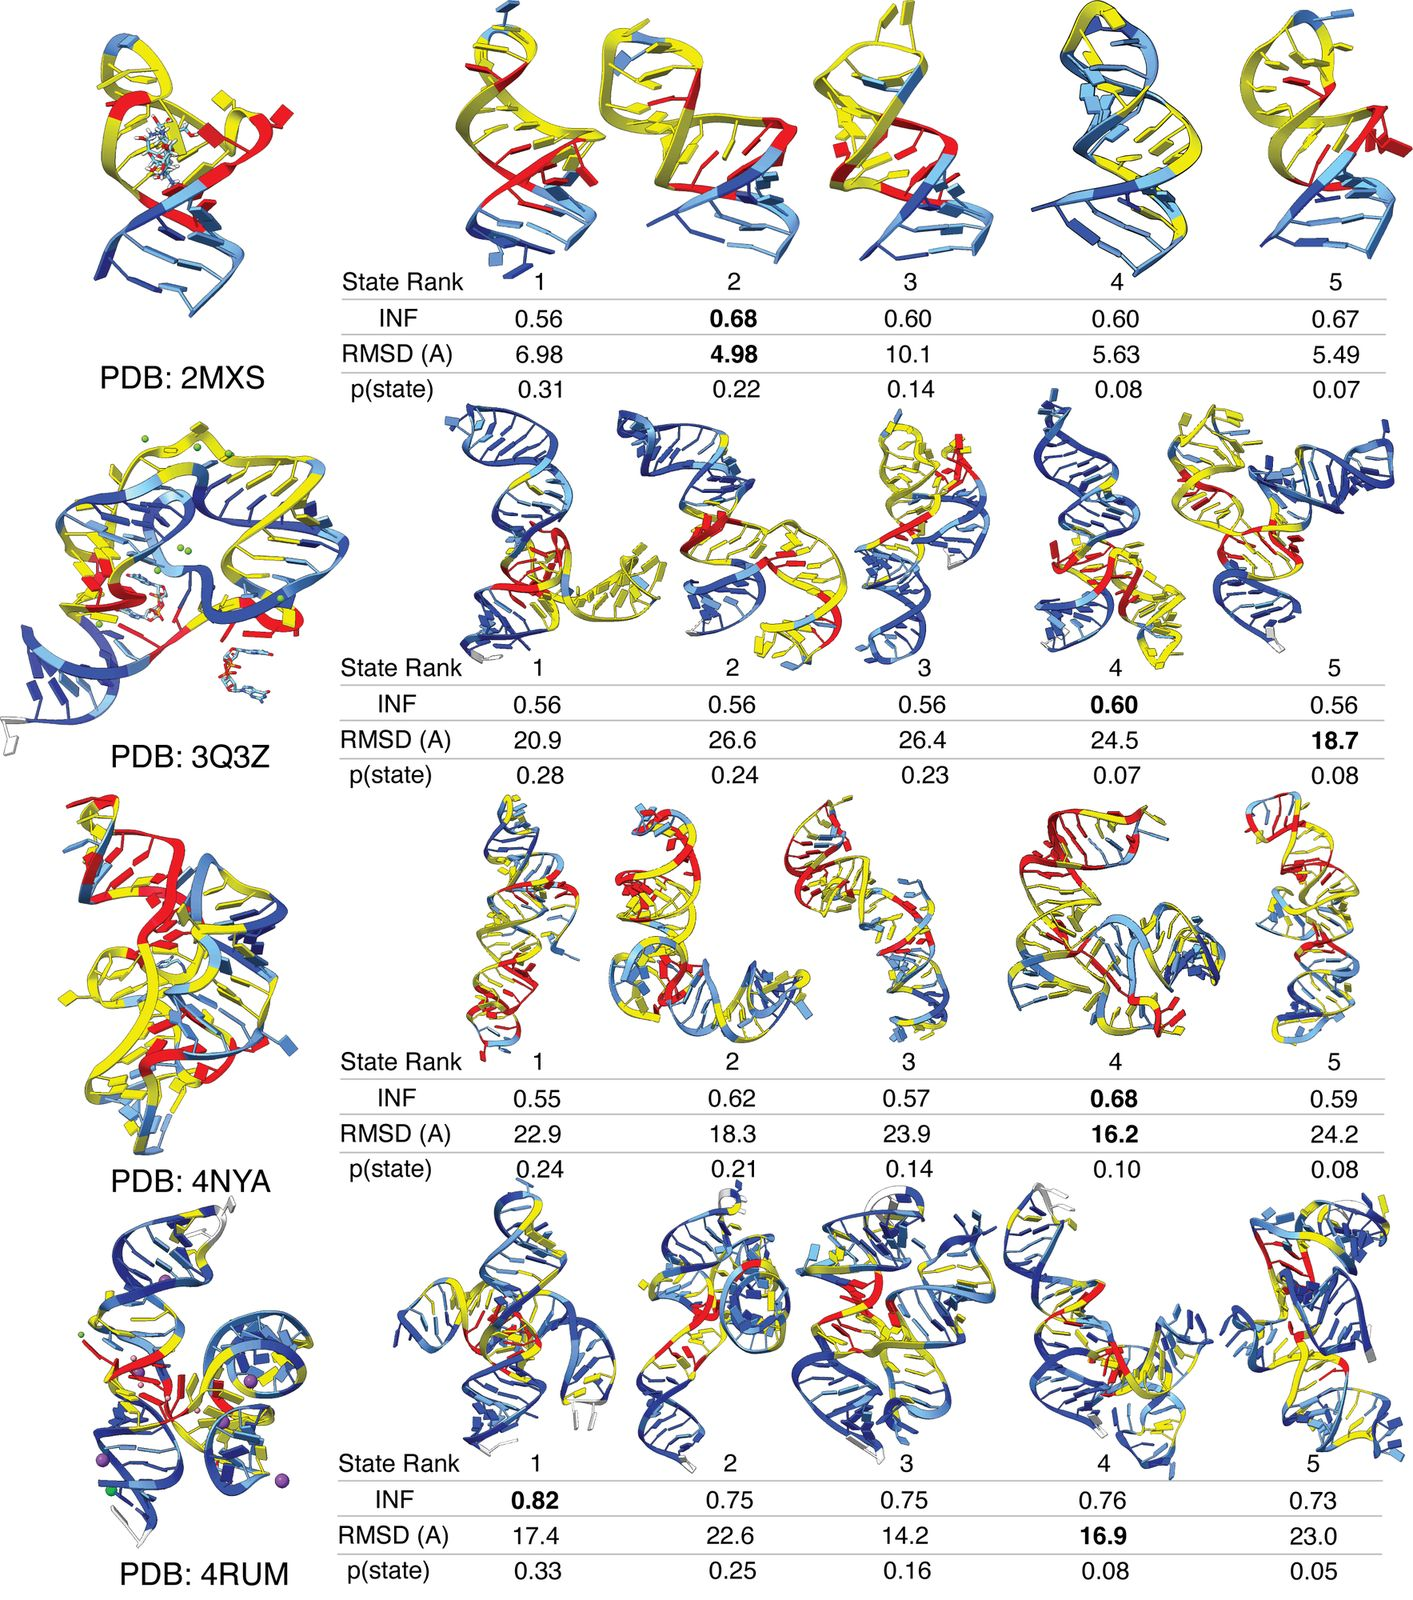
\includegraphics[
    width=\textwidth
    ]{figures/ch6_IE-rep-ensemble-1.jpg}
    \caption[Conformational ensembles predicted by RNAnneal, set 1.]{{\bf Conformational ensembles predicted by RNAnneal (2MXS, 3Q3Z~\cite{Smith2010}, 4NYA~\cite{Warner2014}, 4RUM~\cite{Ramesh2014})}. The reference ERC for each RNA are depicted to the left. The five most probable states are reported alongside their probabilities. The best scoring model from each state is shown as a representative conformation, and the INF and RMSD values compared to the ERC are reported. Nucleotides are colored based on the interaction entropy (IE) predicted by RNAnneal according to the ranges marked in Fig. \ref{ch6:fig:ensemble-results}b (dark blue: $0 \leq \mathrm{IE} < 0.5$; light blue: $0.5 \leq \mathrm{IE} < 1.5$; yellow: $1.5 \leq \mathrm{IE} < 2.5$; red: $ \mathrm{IE} \geq 2.5$)}
    \label{ch6:fig:rep-ensemble-1}%
\end{figure*}

\begin{figure*}
    \centering
    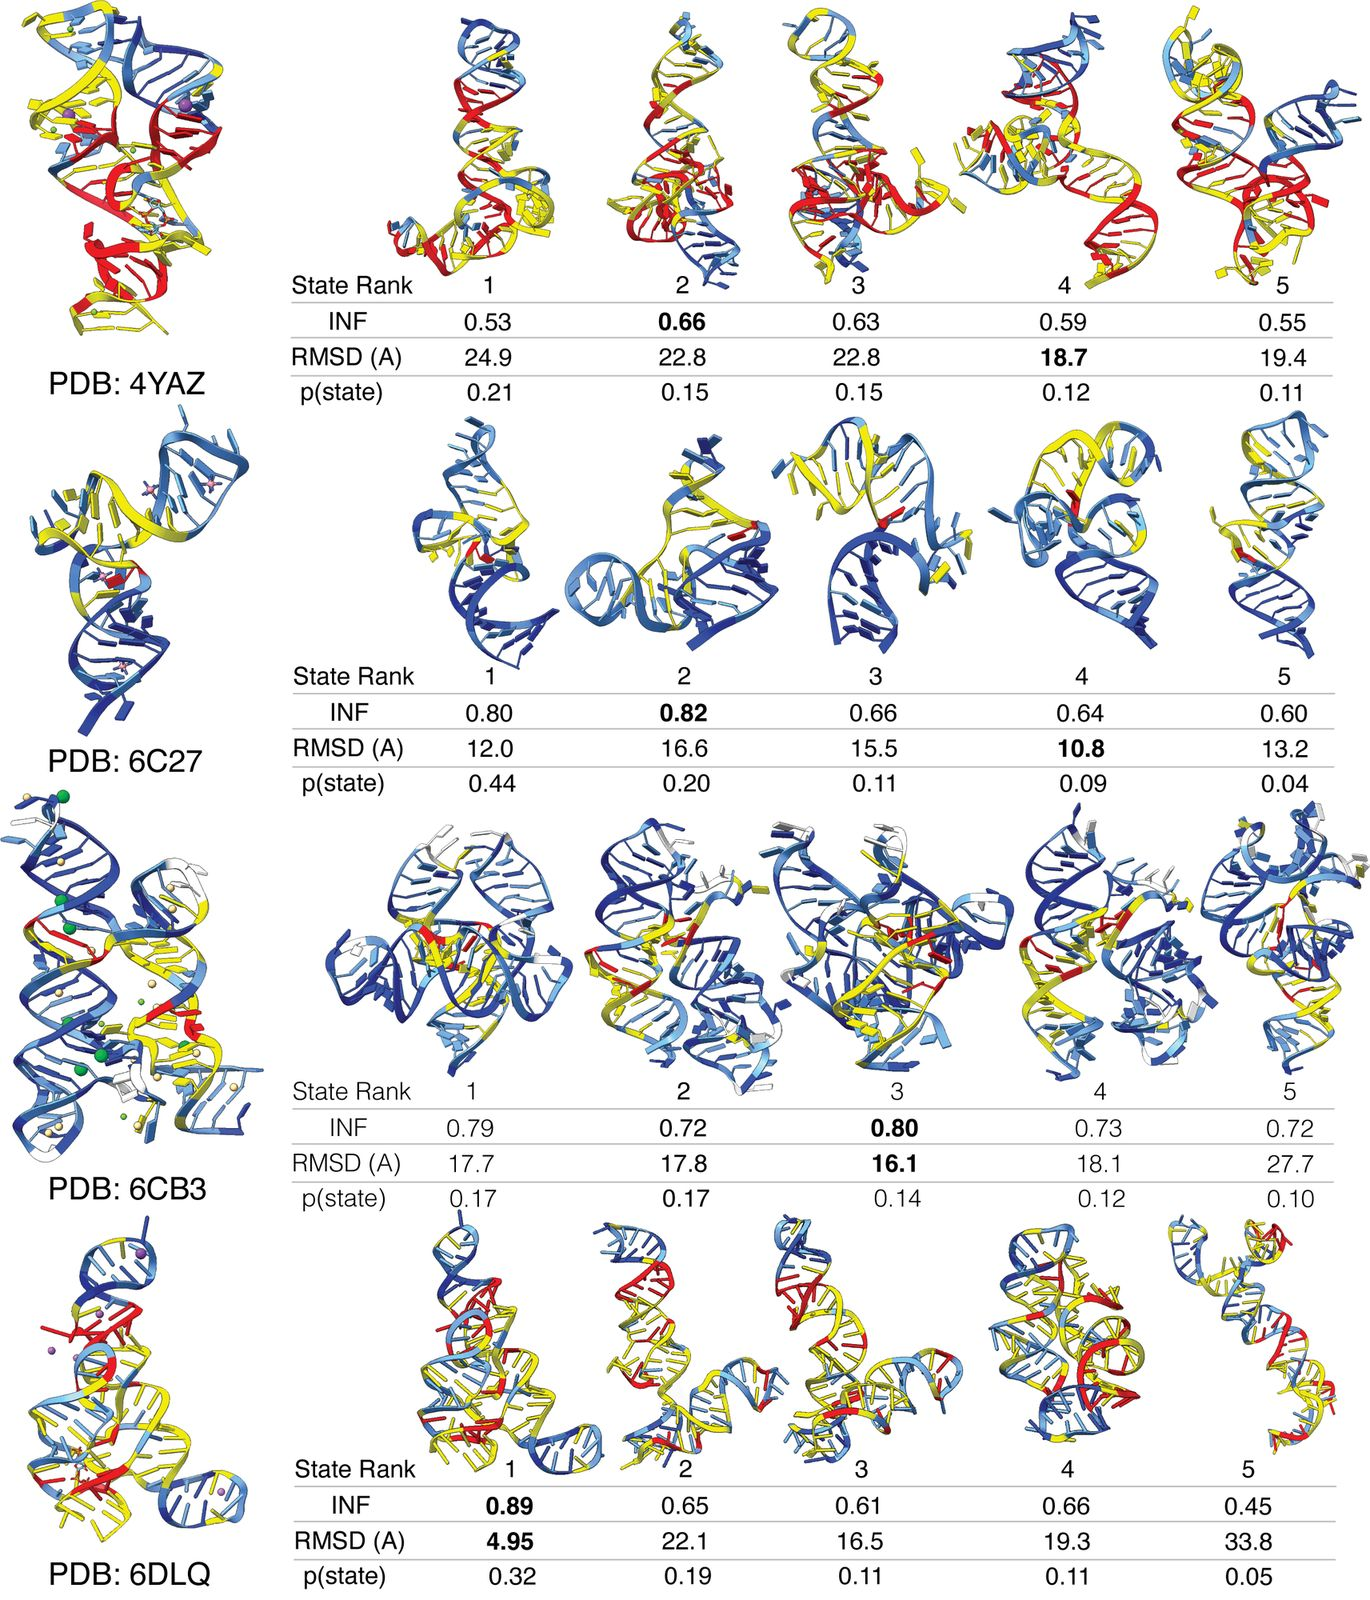
\includegraphics[
    width=\textwidth
    ]{figures/ch6_IE-rep-ensemble-2.jpg}
    \caption[Conformational ensembles predicted by RNAnneal, set 2.]{{\bf Conformational ensembles predicted by RNAnneal (4YAZ~\cite{ren2015structural}, 6C27~\cite{Grigg2018}, 6CB3~\cite{Bachas2018}, 6DLQ~\cite{Peselis2018})}. The reference ERC for each RNA are depicted to the left. The five most probable states are reported alongside their probabilities. The best scoring model from each state is shown as a representative conformation, and the INF and RMSD values compared to the ERC are reported. Nucleotides are colored based on the interaction entropy (IE) predicted by RNAnneal according to the ranges marked in Fig. \ref{ch6:fig:ensemble-results}b (dark blue: $0 \leq \mathrm{IE} < 0.5$; light blue: $0.5 \leq \mathrm{IE} < 1.5$; yellow: $1.5 \leq \mathrm{IE} < 2.5$; red: $ \mathrm{IE} \geq 2.5$)}
    \label{ch6:fig:rep-ensemble-2}%
\end{figure*}

\begin{figure*}
    \centering
    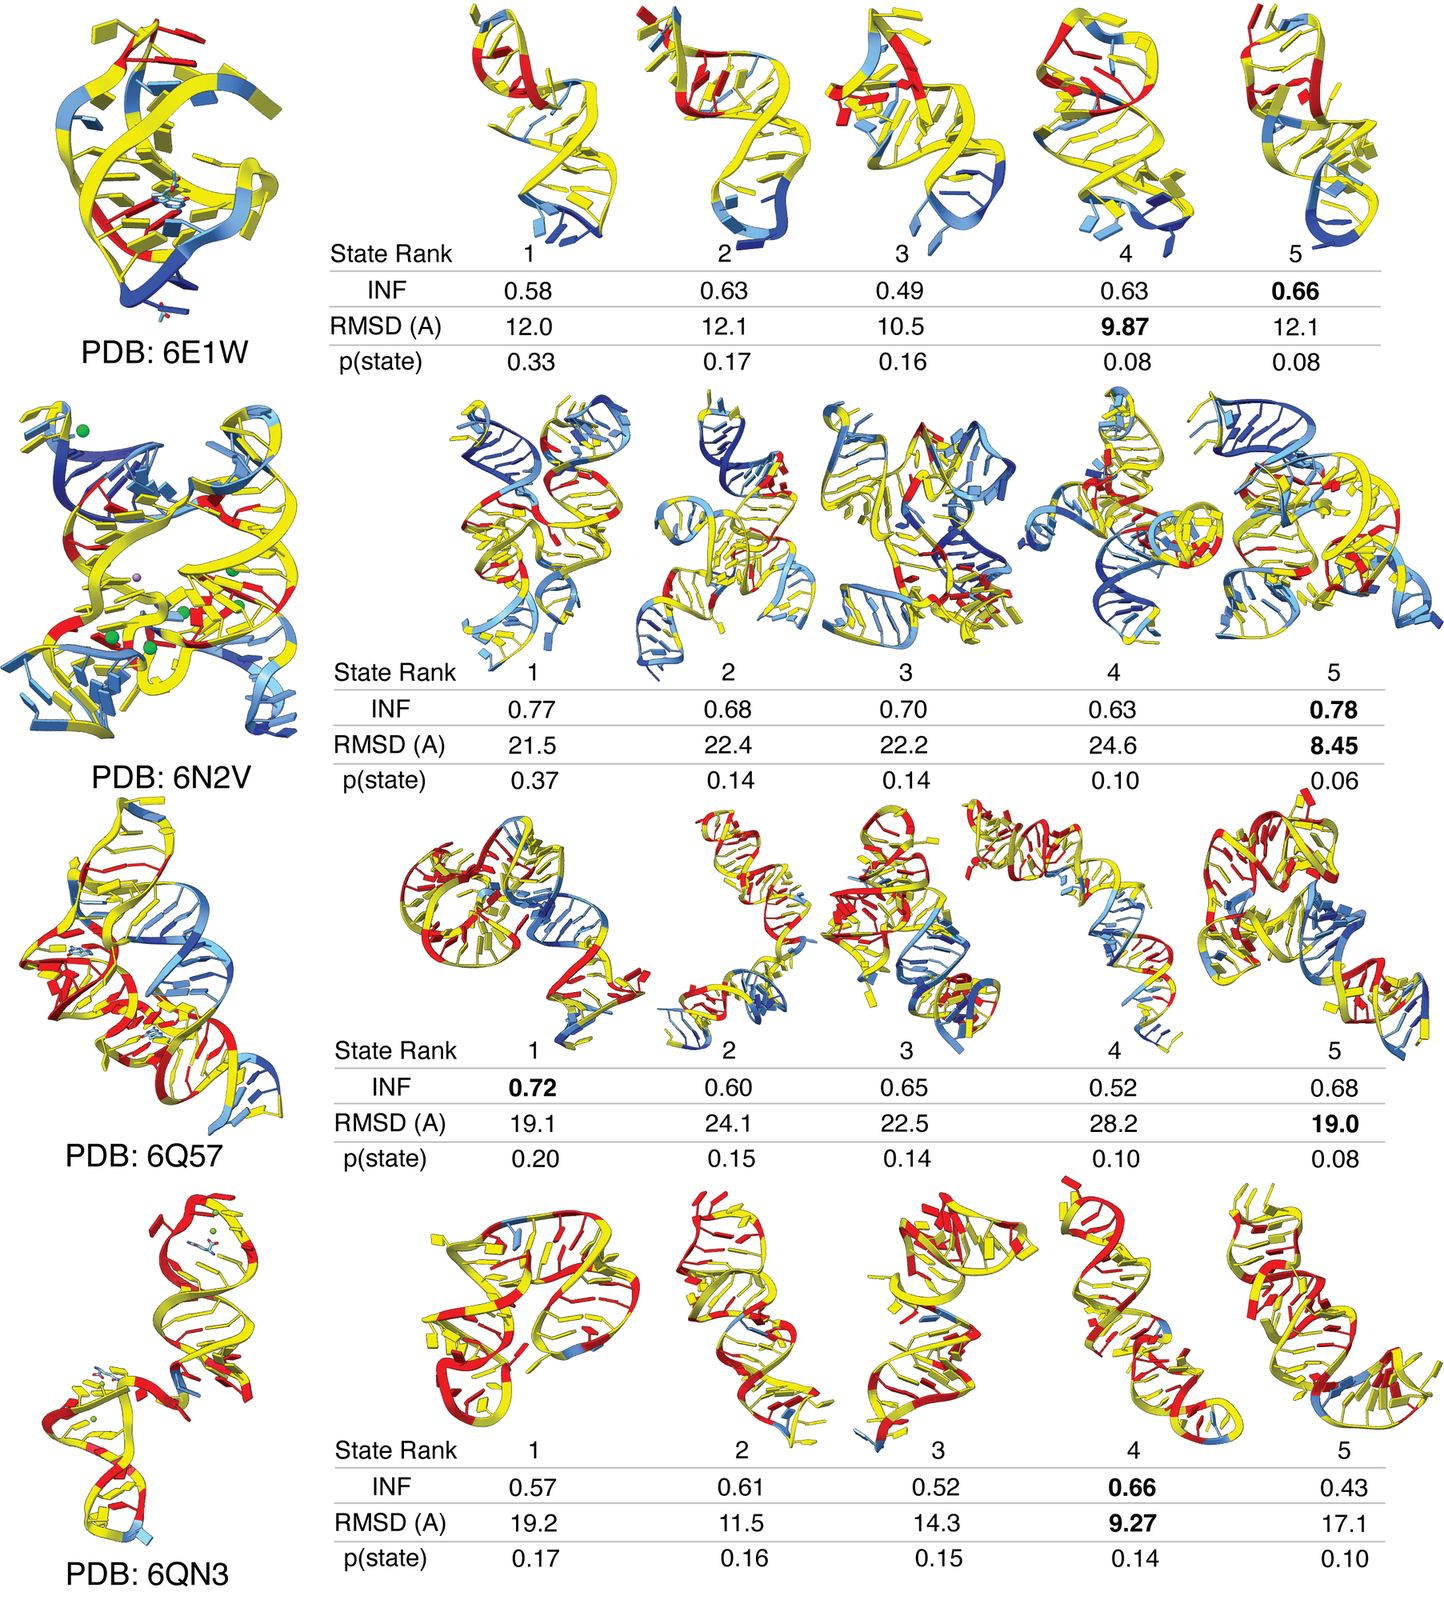
\includegraphics[
    width=\textwidth
    ]{figures/ch6_IE-rep-ensemble-3.jpg}
    \caption[Conformational ensembles predicted by RNAnneal, set 3.]{{\bf Conformational ensembles predicted by RNAnneal (6E1W~\cite{Numata2019}, 6N2V~\cite{Price2018}, 6Q57~\cite{Dunstan2018}, 6QN3~\cite{Huang2019})}. The reference ERC for each RNA are depicted to the left. The five most probable states are reported alongside their probabilities. The best scoring model from each state is shown as a representative conformation, and the INF and RMSD values compared to the ERC are reported. Nucleotides are colored based on the interaction entropy (IE) predicted by RNAnneal according to the ranges marked in Fig. \ref{ch6:fig:ensemble-results}b (dark blue: $0 \leq \mathrm{IE} < 0.5$; light blue: $0.5 \leq \mathrm{IE} < 1.5$; yellow: $1.5 \leq \mathrm{IE} < 2.5$; red: $ \mathrm{IE} \geq 2.5$)}
    \label{ch6:fig:rep-ensemble-3}%
\end{figure*}

\begin{figure*}
    \centering
    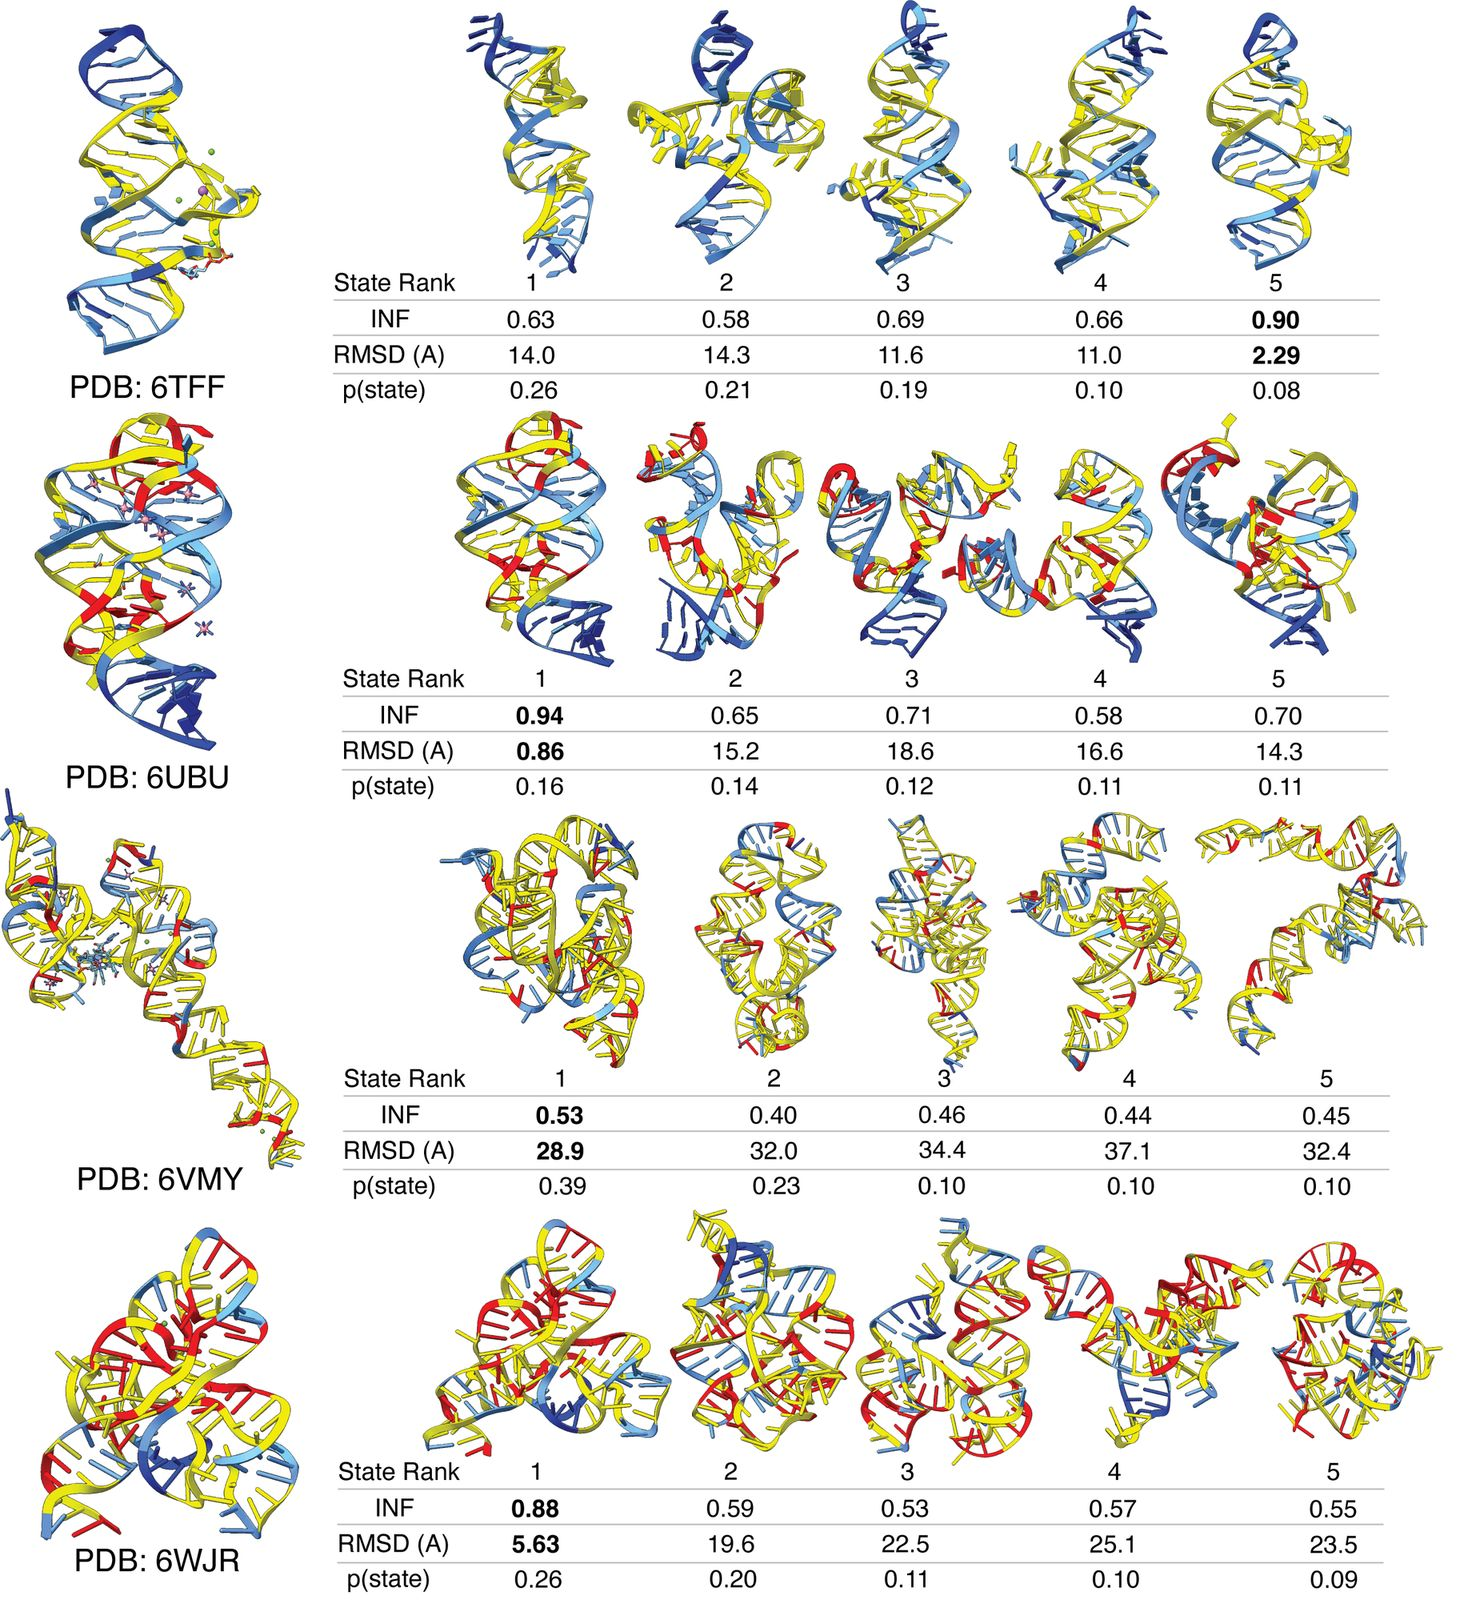
\includegraphics[
    width=\textwidth
    ]{figures/ch6_IE-rep-ensemble-4.jpg}
    \caption[Conformational ensembles predicted by RNAnneal, set 4.]{{\bf Conformational ensembles predicted by RNAnneal (6TFF~\cite{Huang2020}, 6UBU~\cite{Matyjasik2019}, 6WJR~\cite{Wilt2020}, and 6VMY~\cite{Chan2020})}. The reference ERC for each RNA are depicted to the left. The five most probable states are reported alongside their probabilities. The best scoring model from each state is shown as a representative conformation, and the INF and RMSD values compared to the ERC are reported. Nucleotides are colored based on the interaction entropy (IE) predicted by RNAnneal according to the ranges marked in Fig. \ref{ch6:fig:ensemble-results}b (dark blue: $0 \leq \mathrm{IE} < 0.5$; light blue: $0.5 \leq \mathrm{IE} < 1.5$; yellow: $1.5 \leq \mathrm{IE} < 2.5$; red: $ \mathrm{IE} \geq 2.5$)}
    \label{ch6:fig:rep-ensemble-4}%
\end{figure*}

\begin{table}[ht]
  \centering
  \begin{tabular}{@{} l c c c c c c @{}}
    \toprule
    \textbf{RNA} 
      & \textbf{PDB} 
      & \makecell[l]{\textbf{Monomer}}
      % & \textbf{Apo/Holo}
      & \makecell[l]{\textbf{State}}
      & \textbf{Length} 
      & \textbf{Sequence} 
      & \textbf{Secondary Structure} \\
    \midrule
    
    \addlinespace[0.5em]

    % first row
    \makecell[l]{Neomycin \\ sensing \\ riboswitch}
    & 2MXS~\cite{Schmidtke2015}
    & Y
    & Holo
    & 28
    & \makecell[l]{%
          \texttt{ggcugcuuguccuuuaaugguccaguc}
        }
    & \makecell[l]{
      \texttt{(.(((...(.((......)).)))).)}
      } \\

    \addlinespace[0.5em]

    % second row
    \makecell[l]{c‑di‑GMP‑II \\ riboswitch}
    & 3Q3Z~\cite{Smith2010}
    & Y
    & Holo
    & 76
    & \makecell[l]{%
          \texttt{gcgcggaaacaaugaugaauggguuuaaau}  \\
          \texttt{ugggcacuugacucauuuugaguuaguagu} \\
          \texttt{gcaaccgaccgugcu}
          }
    & \makecell[l]{
      \texttt{((.(((..((.......((((.((......}\\
      \texttt{[\{\{[[[[[..)).))))....))....]]]}\\
      \texttt{]]].\}\}..))).)).}
      }
      \\

    \addlinespace[0.5em]

    \makecell[l]{TPP \\ riboswitch}
    & 4NYA~\cite{Warner2014}
    & Y
    & Holo
    & 81
    & \makecell[l]{%
          \texttt{ggacucggggugcccuucugcgugaaggcu} \\
          \texttt{gagaaauacccguaucaccugaucuggaua} \\ 
          \texttt{augccagcguagggaaguuc} \\
        }
      
    & \makecell[l]{
    \texttt{(.(((((((.((((.(((.....)))))).}\\
    \texttt{.....)..)))).....(((...((((...}\\
    \texttt{...))))...)))..))).)}
      }
      \\

        \addlinespace[0.5em]

    \makecell[l]{NiCo \\ transition\\-metal \\ riboswitch}
    & 4RUM~\cite{Warner2014}
    & Y
    & Holo
    & 93
    & \makecell[l]{%
          \texttt{gggaacugagcaggcaaugaccagagcggu} \\
          \texttt{caugcagccgggcugcgaaagcggcaacag} \\
          \texttt{augauacacgcacaucugugggacaguucc} \\
          \texttt{ca}
        }

    & \makecell[l]{
    \texttt{((((((((..(.(((.((((((.....)))} \\
    \texttt{)))...)))..((.((....)).)).((((} \\
    \texttt{(((.........)))))))..).)))))))} \\
    \texttt{).}
      }
      \\

    \addlinespace[0.5em]

        \makecell[l]{3',3'-cGAMP \\ sensing \\ riboswitch}
    & 4YAZ~\cite{ren2015structural}
    & Y
    & Holo
    & 84
    & \makecell[l]{%
          \texttt{gguacacgacaauacuaaaccauccgcgag} \\
          \texttt{gauggggcggaaagccuaagggucucccug} \\
          \texttt{agacagccgggcugccgaaauauc}
        }

    & \makecell[l]{
    \texttt{(.((..((......(....((((((....)} \\
    \texttt{)))))..[.)...(((...(((((((...)} \\
    \texttt{)))).])).)))...))...)).)} \\
    }
      \\

    \addlinespace[0.5em]

    \makecell[l]{SAM-III \\ riboswitch}
    & 6C27~\cite{Grigg2018}
    & Y
    & Apo
    & 48
    & \makecell[l]{%
          \texttt{gggacaaguucccgaaaggauggcggaaac} \\
          \texttt{gccagaugccuuguccc} \\
        }

    & \makecell[l]{
    \texttt{.(((((((.(.(.....).)(.((......} \\
    \texttt{)).).....))))))).} \\
      }
      \\

    \addlinespace[0.5em]

    \makecell[l]{YkoY\\riboswitch}
    & 6CB3~\cite{Bachas2018}
    & N
    & Holo
    & 100
      & \makecell[l]{%
          \texttt{aaaggggaguagcgucgggaaaccgaaaca} \\
          \texttt{aagucgucaauucgugaggaaacucaccgg} \\
          \texttt{cuuuguugacauacgaaaguauguuuagca} \\
          \texttt{agaccuuuc} \\
        }
      & \makecell[l]{
    \texttt{.((((......((.((((....))))((((} \\
    \texttt{(((.((.......(((((....))))))).} \\
    \texttt{))))))).((((((....))))))...)).} \\
    \texttt{...))))..} \\
      }
      \\

    \addlinespace[0.5em]

    \makecell[l]{PRPP \\ riboswitch}
    & 6DLQ~\cite{Peselis2018}
    & Y
    & Holo
    & 108
    & \makecell[l]{%
          \texttt{ggaaagugugucuaggguuccgcgugcuuc} \\
          \texttt{ggcacggacugguccaagugacacagacgc} \\
          \texttt{auucgugcguuacaccggagggauagaagc} \\
          \texttt{ccaggcggguagguuuc} \\
        }
    & \makecell[l]{
    \texttt{..((...(((((..((...((.(((((...} \\
    \texttt{.)))))....)).))....)))))..((((} \\
    \texttt{(....)))))..(.[[[..(((.......)} \\
    \texttt{)).).]]]......)).} \\
      }
      \\

    \addlinespace[0.5em]

    \makecell[l]{PreQ1 \\ riboswitch}
    & 6E1W~\cite{Numata2019}
    & Y
    & Holo
    & 31
    & \makecell[l]{%
          \texttt{cugggucgcaguuuccccaguuaacaaaac}
        }
    & \makecell[l]{
    \texttt{(((((.....[....))))).........]}
      }
      \\

    \addlinespace[0.5em]

    \makecell[l]{Mn$^{2+}$-\\sensing \\ riboswitch}
    & 6N2V~\cite{Price2018}
    & Y
    & Holo
    & 99
    & \makecell[l]{%
          \texttt{gcuuggggaguagccugcuuucggaaacga} \\
          \texttt{aagcgccuguaucaacauacucggcgaaag} \\
          \texttt{ccguggugcaggaccgaaaggucuggcgag} \\
          \texttt{accaggcc}
        }

    & \makecell[l]{
    \texttt{.(.(((......(((..(.((((....)))} \\
    \texttt{).)..((((.(.((.......((((....)} \\
    \texttt{))))).).))))(((....)))..)))...} \\
    \texttt{.))).)..} \\
      }
      \\

    \addlinespace[0.5em]

    \makecell[l]{Tetrahydro-\\folate \\ riboswitch}
    & 6Q57~\cite{Dunstan2018}
    & Y
    & Holo
    & 90
    & \makecell[l]{%
          \texttt{ggagaguagaugauucgcguuaagugugug} \\
          \texttt{ugaaugggaugucgucacacaacgaagcga} \\
          \texttt{gagcgcggugaaucauugcauccgcucca} \\
        }
      
    & \makecell[l]{
    \texttt{.(((......((((((.((.......((((} \\
    \texttt{(((...[[[[[...)))))))....((...} \\
    \texttt{.)).))..))))))...]]]]].)))..} \\
      }
      \\

    \addlinespace[0.5em]

    \makecell[l]{Glutamine \\ II riboswitch}
    & 6QN3~\cite{Huang2019}
    & N
    & Holo
    & 51
    & \makecell[l]{%
          \texttt{cguucacccuucggggcgcaugaaauggga} \\
          \texttt{guagggaacgggauucucau}
        }
    & \makecell[l]{
    \texttt{......(((....)))........(.(.((} \\
    \texttt{.(..........).)).).)} \\
      }
      \\

    \addlinespace[0.5em]

    \makecell[l]{NAD$^{+}$ \\ riboswitch}
    & 6TFF~\cite{Huang2020}
    & Y
    & Holo
    & 53
    & \makecell[l]{%
          \texttt{ggcuucaacaaccccguagguugggccgaa} \\
          \texttt{aggcagcgaaucuacuggagcc}
        }
    & \makecell[l]{
    \texttt{((((.((.....[[.((((.(((.(((...} \\
    \texttt{.))).]]))).)))))).))))} \\
      }
      \\

    \addlinespace[0.5em]

    \makecell[l]{Guanine\\ riboswitch}
    & 6UBU~\cite{Matyjasik2019}
    & Y
    & Holo
    & 68
    & \makecell[l]{%
          \texttt{ggacauauaaucgcguggauauggcacgca} \\
          \texttt{aguuucuaccgggcaccguaaauguccgac} \\
          \texttt{uaugucc}
        }

    & \makecell[l]{
    \texttt{((((((((..(.(((((.....[[))))).} \\
    \texttt{)[.....)](((.((]].....)).)))..} \\
    \texttt{)))))))} \\
      }
      \\

    \addlinespace[0.5em]

    \makecell[l]{FMN \\ riboswitch}
    & 6WJR~\cite{Wilt2020}
    & Y
    & Apo
    & 112
    & \makecell[l]{%
          \texttt{ggaucuucggggcagggugaaauucccgac} \\
          \texttt{cggugguauaguccacgaaaguauuugcuu} \\
          \texttt{ugauuuggugaaauuccaaaaccgacagua} \\
          \texttt{gagucuggaugagagaagauu}
        }
    & \makecell[l]{
    \texttt{..((((((.......((.......))..((} \\
    \texttt{((((((....[[))))..(((......)))} \\
    \texttt{...(((((.......)))))]])).[[[..} \\
    \texttt{..))]]].......)))))).} \\
      }
      \\
    
    \addlinespace[0.5em]

    \makecell[l]{Cobalamin \\ riboswitch}
    & 6VMY~\cite{Chan2020}
    & Y
    & Holo
    & 149
    & \makecell[l]{%
          \texttt{ggucaaauaggugccgguccgugaacaaca} \\
          \texttt{gccggcuuaaaagggaaaccgguaaaagcc} \\
          \texttt{ggugcggucccgccacuguaauuggccaag} \\
          \texttt{cgccaagagccaggauaccugccuguuuga} \\
          \texttt{ucagcacgaauucugcgaggacagauga}
        }
    & \makecell[l]{
    \texttt{(.((.((.(((.(((((..[((.....)).} \\
    \texttt{.))))).....(((....((((......))} \\
    \texttt{)).((((.....)).[[[....((((....} \\
    \texttt{.))))...))]]]]...))).))).)).))} \\
    \texttt{.)..(.....((........).)...).} \\
      }
      \\

    \bottomrule
  \end{tabular}
  \caption{Details of riboswitch sequences and reference conformations}
  \label{ch6:tab:riboswitches}
\end{table}

\begin{table}[]
  \centering
  \begin{tabular}{lccc}
    \toprule
    \textbf{Stage} & \textbf{Duration (ps)} & \textbf{Timestep (fs)} & \textbf{Temperature (K)} \\
    \midrule
    Equilibration 1   &     1    &  0.1 &   1   \\
    Equilibration 2.1 &     1    &    1 &  10   \\
    Equilibration 2.2 &     1    &    1 &  20   \\
    Equilibration 2.3 &     1    &    1 &  30   \\
    Equilibration 2.4 &     1    &    1 &  40   \\
    Equilibration 2.5 &     1    &    1 &  50   \\
    Equilibration 3.1 &     2    &    1 & 100   \\
    Equilibration 3.2 &     2    &    1 & 150   \\
    Equilibration 3.3 &     2    &    1 & 200   \\
    Equilibration 3.4 &     2    &    1 & 250   \\
    Equilibration 3.5 &     2    &    1 & 300   \\
    Equilibration 4.1 &    20    &    1 & 300   \\
    Equilibration 4.2 &    20    &    2 & 300   \\
    Equilibration 4.3 &    20    &    3 & 300   \\
    Equilibration 4.4 &    20    &    4 & 300   \\
    Equilibration 4.5 &    20    &    5 & 300   \\
    Production        & 100{,}000 &    5 & 300   \\
    \bottomrule
  \end{tabular}
    \caption{Molecular Dynamics Equilibration Procedure}
  \label{ch6:tab:schedule}
\end{table}

\begin{table}[]
  \centering
  \begin{tabular}{ll}
    \toprule
    \textbf{Parameter}            & \textbf{Value}                    \\
    \midrule
    Simulation Engine             & OpenMM                            \\
    Ion Type                      & NaCl                              \\
    Ion Concentation              & 1 M                                \\
    Box Shape                     & Dodecahedron                      \\
    Box Padding                   & 0.5 nm                            \\
    Force Field (Solute)           & RNA.Shaw\_charmm22-ions.xml       \\
    Force Field (Solvent)          & implicit/gbn2.xml                 \\
    Pressure                      & 1 atm                             \\
    Sampling Frequency            & 1 ns                              \\
    \bottomrule
  \end{tabular}
  \caption{Molecular Dynamics Simulation Parameters.}
\label{ch6:tab:parameters}
\end{table}
